%% =====================================================================
%%  X-UAD : Explainable Hybrid Vision Transformer with Adaptive Quantum
%%          Attention and Evidence-Grounded MLLM Reasoning for Unified
%%          Face Attack Detection
%%  IEEE conference format (IEEEtran).  Compile with pdflatex + bibtex.
%% =====================================================================
\documentclass[conference]{IEEEtran}
\IEEEoverridecommandlockouts

\usepackage{cite}
\usepackage{amsmath,amssymb,amsfonts}
\usepackage{algorithm}
\usepackage{algorithmic}
\usepackage{graphicx}
\usepackage{booktabs}
\usepackage{multirow}
\usepackage{xcolor}
\usepackage{textcomp}
\usepackage[caption=false]{subfig}
\usepackage{url}
\usepackage[hidelinks]{hyperref}

\def\BibTeX{{\rm B\kern-.05em{\sc i\kern-.025em b}\kern-.08em T\kern-.1667em\lower.7ex\hbox{E}\kern-.125emX}}

\newcommand{\bs}[1]{\boldsymbol{#1}}
\newcommand{\R}{\mathbb{R}}
\newcommand{\ket}[1]{\lvert #1 \rangle}
\newcommand{\bra}[1]{\langle #1 \rvert}
\newcommand{\braket}[2]{\langle #1 \vert #2 \rangle}
\newcommand{\up}{$\uparrow$}
\newcommand{\down}{$\downarrow$}

\begin{document}

\title{Explainable Hybrid Vision Transformer with Adaptive Quantum Attention and
Evidence-Grounded Reasoning for Unified Face Attack Detection}

\author{\IEEEauthorblockN{Swethaa Premnath}
\IEEEauthorblockA{\textit{Vellore Institute of Technology} \\
Vellore, India \\
swethaa.premnath2024@vitstudent.ac.in}
}

\maketitle

\begin{abstract}
Face recognition systems are attacked from two directions that the literature has
largely treated as separate problems: \emph{physical} presentation attacks
(printed photographs, replayed video, 3-D masks) and \emph{digital} manipulations
(face-swaps, reenactment, fully synthetic faces, adversarial perturbations). A
detector specialised to one degrades on the other; and whichever it handles, it
returns an uncalibrated scalar, cannot say when an attack falls outside the
families it was trained on, and offers no account of why a face was rejected. We
present \textbf{X-UAD}, a single model that detects both families, reports how much
it does not know, localises the evidence, and explains itself in language that can
be audited line by line. Three ideas make this possible. \emph{Adaptive Quantum
Attention} adds a Born-rule scoring channel --- the squared overlap of
amplitude-encoded token states evolved by parameterised Givens circuits, which are
orthogonal by construction and use $\mathcal{O}(dL)$ angles instead of
$\mathcal{O}(d^{2})$ weights --- gated per head against the classical dot product,
matching the sign-invariant, interference character of moir\'e, halftone and
up-sampling evidence. A learnable orthonormal \emph{quantum evidence basis},
measured against every token, is used simultaneously as a classification feature
and, unchanged, as the explanation, so the rationale is a read-out of the
computation rather than a post-hoc approximation of it. A \emph{decoupled
evidential head} predicts the Dirichlet direction and magnitude separately and is
trained with \emph{pseudo-unseen evidence suppression}, an out-of-taxonomy proxy
manufactured from the attack taxonomy itself. We build a difficulty-calibrated,
identity-disjoint, ID-consistent benchmark of eight attack families with
pixel-level evidence ground truth, and compare against ResNet-18, ViT-Tiny and
CDCN++ re-implemented and trained under an identical budget. On the closed-set
protocol the three convolutional and hybrid detectors are all close to the ceiling
(ACER $0.71$--$1.46\%$, AUC $\approx99.9\%$); X-UAD gives the lowest calibration error of any
model that actually detects ($1.94\%$ ECE, against $2.11\%$ and $3.44\%$; the plain
transformer's $0.67\%$ is the degenerate calibration of a near-chance classifier)
and the best evidence localisation ($77.8\%$ region-level IoU), while trailing the
best baseline by $0.75$ ACER points. Under leave-one-attack-out it
attains the best mean detection rate on families it has never seen ($77.5\%$) and
the best novelty AUROC on half the folds, and pseudo-unseen suppression is worth
$+5.4$ AUROC points on that channel. We also report a negative result the field
should know: under a severe capture-domain shift \emph{every} method in the
comparison collapses. Code, benchmark generator and configurations that map the
identical pipeline onto the public capture-based corpora are released.
\end{abstract}

\begin{IEEEkeywords}
face anti-spoofing, presentation attack detection, deepfake detection, unified
attack detection, vision transformer, quantum-inspired attention, evidential deep
learning, uncertainty estimation, open-set recognition, explainable AI
\end{IEEEkeywords}

% =====================================================================
\section{Introduction}
% =====================================================================

A modern face verification pipeline is exposed to two structurally different threat
surfaces. In front of the sensor an adversary can hold up a printed photograph,
replay a video on a phone, or wear a silicone mask; these are
\emph{physical presentation attacks} (PAs) and they leave traces of a
\emph{re-acquisition process}: halftone screening, a display sub-pixel lattice
aliasing into moir\'e, specular sheen, lost skin micro-texture. Behind the sensor
an adversary can swap an identity, drive an expression, synthesise a face outright,
or add an imperceptible gradient-crafted perturbation; these are \emph{digital
attacks} and they leave traces of a \emph{generative process}: blending boundaries,
resolution mismatch, up-sampling checkerboards, anisotropic peaks in the Fourier
magnitude.

Because the two evidence types look nothing alike, the two research communities
grew apart. Face anti-spoofing (FAS) built texture- and depth-driven detectors
\cite{liu2018auxiliary,yu2020cdcn,yu2021revisiting,wang2022ssan}; face forgery
forensics built frequency- and blending-driven detectors
\cite{rossler2019ff,li2020celebdf,frank2020frequency,wang2020cnnspot}. Deploying
both is not a solution: a system needs one decision, one threshold and one audit
trail, and a two-model cascade doubles the calibration burden while leaving the
question of what to do when the two heads disagree. The recent unified
physical--digital line of work
\cite{yu2024unified,yuan2024challenge,ma2025uniattackplus,chen2025uniattack,zhang2024unidefense}
recognised this and produced ID-consistent corpora and joint detectors. Its own
results, however, expose the remaining problem: on the seen-attack protocol of
UniAttackData every reasonable method is essentially saturated (ACER $\approx
0.5$--$1.4\%$), whereas on the protocol that withholds attack families the same
methods collapse to ACER $22$--$44\%$ with double-digit standard deviations
\cite{yu2024unified}. Unified detection is therefore not solved; it is solved
\emph{in-distribution} and unsolved \emph{out-of-distribution}.

Three further capabilities are absent from essentially all of this work, and all
three are what an operator actually needs when the score is ambiguous:

\begin{enumerate}
\item \textbf{A usable notion of ``I do not know''.} A softmax score is a
      \emph{closed-set} quantity: it redistributes probability over the classes it
      was trained on, so a wholly novel attack can be assigned $99\%$ confidence to
      the nearest known family. What is needed is a second-order belief that can be
      \emph{vacuous}.
\item \textbf{Evidence localisation.} Pixel-wise FAS supervises a depth or binary
      map \cite{yu2021revisiting,liu2018auxiliary}, but depth is a proxy for
      liveness, not a map of the forensic evidence, and it is meaningless for
      digital attacks.
\item \textbf{An explanation that is bound to the decision.} Multimodal-LLM
      forensics \cite{huang2024ffaa,guo2025m2f2det} produces fluent narratives, but
      the language model does not observe the detector's internal state, so its
      narrative is at best correlated with the decision, and its specifics (``a
      visible screen bezel'') are unverifiable and frequently absent from the
      frame.
\end{enumerate}

\noindent\textbf{This paper.} We present X-UAD, a single model that detects
physical and digital attacks jointly, estimates how much it does not know,
localises the evidence, and explains itself in language that can be audited. Our
contributions are:

\begin{itemize}
\item \textbf{Adaptive Quantum Attention (AQA).} Classical attention scores a pair
      of tokens by an unbounded \emph{linear} functional. Much of the evidence for
      face attacks is an \emph{interference} phenomenon --- a moir\'e beat, a
      checkerboard, a spectral peak --- which is visible in the squared modulus of a
      projection, not in the projection. AQA adds a Born-rule channel:
      $S_{ij}=|\braket{\psi^{Q}_{i}}{\psi^{K}_{j}}|^{2}$ between amplitude-encoded
      token states evolved by parameterised Givens circuits, mixed into the
      classical channel by a per-head, input-conditioned gate. The circuits are
      exactly orthogonal by construction and are parameterised by
      $\mathcal{O}(dL)$ angles instead of $\mathcal{O}(d^{2})$ weights.
\item \textbf{A quantum evidence basis that makes the explanation intrinsic.} A
      learnable \emph{orthonormal} basis (the image of the computational basis under
      a Givens circuit, so orthonormality holds exactly at every training step) is
      measured against every spatial token. The resulting Born probabilities are a
      token$\times$mode evidence spectrum that is used \emph{both} as a
      classification feature and, unchanged, as the explanation --- so the
      explanation is a read-out of the computation rather than a post-hoc
      approximation of it.
\item \textbf{Pseudo-Unseen Evidence Suppression (PUES).} Convex mixtures of two
      \emph{different} attack families are, by construction, outside the taxonomy:
      no single physical or generative process produces a superposition of two
      signatures. Driving the Dirichlet evidence of such mixtures to zero teaches
      the vacuity channel what ``unseen'' looks like without ever showing the model
      a real unseen attack, and turns vacuity from a calibration statistic into a
      usable open-set score.
\item \textbf{Evidence-grounded reasoning.} A forward pass emits a typed, numeric
      \emph{evidence record}; language is generated only from that record. The
      deterministic realiser has zero hallucination by construction; an optional
      hosted-MLLM back-end is constrained by the same record and its output is
      re-verified against it. The end product is the operator verdict
      \texttt{Attack / Confidence / Risk} plus a traceable rationale.
\item \textbf{A difficulty-calibrated, ID-consistent unified benchmark} of eight
      families with \emph{pixel-level evidence ground truth} --- a supervision and
      evaluation signal that no capture-based PAD corpus provides --- together with
      identity-disjoint, leave-one-attack-out and cross-domain protocols, and an
      explicit calibration procedure that prevents the trivially separable regime
      that inflates simulated benchmarks.
\end{itemize}

Section~\ref{sec:related} surveys the four lines of work X-UAD unifies and states
the research gap explicitly (Table~\ref{tab:gap}); Section~\ref{sec:bench}
describes the benchmark; Section~\ref{sec:method} the model;
Section~\ref{sec:exp} the experiments; Section~\ref{sec:gap} returns to the gap and
states, component by component, how it is closed.

% =====================================================================
\section{Related Work and the Research Gap}\label{sec:related}
% =====================================================================

\subsection{Physical presentation attack detection}
Early FAS treated liveness as a texture problem. Auxiliary supervision
\cite{liu2018auxiliary} replaced the binary label with a pseudo-depth map and rPPG
signal; Central Difference Convolution (CDC) \cite{yu2020cdcn} made the first
layers respond to illumination-invariant micro-texture by mixing the local gradient
into the convolution, and remains the strongest lightweight backbone for physical
PAs. Pixel-wise supervision was systematically revisited in \cite{yu2021revisiting}.
Generalisation across capture domains was attacked with adversarial domain
generalisation \cite{shao2019mada}, single-side domain generalisation
\cite{jia2020ssdg} and style-shuffled separation \cite{wang2022ssan}. All of these
assume the attack is in front of the camera; none has a mechanism for a digitally
manipulated but physically genuine capture.

\subsection{Digital forgery detection}
FaceForensics++ \cite{rossler2019ff} and Celeb-DF \cite{li2020celebdf} established
the benchmarks. The most transferable cues turned out to be spectral: generators
leave periodic up-sampling artefacts \cite{odena2016checkerboard} that show up as
characteristic peaks in the Fourier magnitude \cite{frank2020frequency}, which is
why simple detectors generalise surprisingly far across generators
\cite{wang2020cnnspot}. These detectors, symmetrically, have no notion of a
re-acquisition medium and fail on print and replay.

\subsection{Unified physical--digital detection}
UniAttackData \cite{yu2024unified} is the pivotal contribution: an
\emph{ID-consistent} corpus in which the same subject appears as bonafide and under
every attack, so identity cannot be used as a shortcut, together with
UniAttackDetection, a vision-language detector with teacher--student prompts and
unified knowledge mining. The CVPR'24 and ICCV'25 challenges
\cite{yuan2024challenge,ma2025uniattackplus} scaled this to $2{,}875$ subjects and
$54$ attack types and confirmed two things: methods built on large pre-trained
multimodal backbones dominate, and single-modality CNNs are stuck above $20\%$
ACER. UniDefense \cite{zhang2024unidefense} approaches the same goal through dual
space reconstruction. What none of these systems provides is an uncertainty
channel, an evidence map, or an explanation: the output is a score.

\subsection{Uncertainty and open-set recognition}
Maximum-softmax-probability \cite{hendrycks2017msp} is a weak out-of-distribution
score precisely because softmax is closed-set. Prior networks
\cite{malinin2018prior} and evidential deep learning \cite{sensoy2018edl}, built on
subjective logic \cite{josang2016subjective}, place a Dirichlet over the simplex so
that total evidence --- and therefore \emph{vacuity} --- is representable.
Outlier exposure \cite{hendrycks2019oe} shows that a proxy for ``other'' is worth
more than any purely intrinsic score. Open-set single-domain generalisation has
recently been posed for FAS \cite{liu2024openset}, but evidential uncertainty has
not been combined with unified physical--digital detection, and no prior work
constructs its outlier proxy \emph{from the attack taxonomy itself}.

\subsection{Explainability and MLLM forensics}
Attention rollout \cite{abnar2020rollout} and deletion/insertion faithfulness
\cite{petsiuk2018rise} are the standard tools for asking whether an explanation
reflects a decision. FFAA \cite{huang2024ffaa} fine-tunes an MLLM for open-world
face forgery analysis with a multi-answer decision system; M2F2-Det
\cite{guo2025m2f2det} bridges CLIP and an LLM for interpretable forged-face
detection. Both generate fluent text, and both are \emph{post-hoc narrators}: the
language model is not given the detector's internal evidence, so its account cannot
be checked against the decision and it is free to assert artefacts that are not
present.

\subsection{Quantum-inspired attention}
Quantum Vision Transformers \cite{cherrat2024qvt} and quantum self-attention
\cite{comajoan2024qgluon,evans2025on} replace linear projections with parameterised
quantum circuits, reporting accuracy comparable to classical ViTs at a small
fraction of the parameters --- the $\mathcal{O}(n^{2})\!\to\!\mathcal{O}(n)$
argument. That literature is motivated by parameter efficiency and is evaluated on
generic classification. It has not been connected to a task whose evidence is
\emph{physically} an interference pattern, and it offers no explainability story.

\subsection{The research gap}
Table~\ref{tab:gap} places the six lines side by side. Every prior system occupies
a proper subset of the required capabilities, and --- crucially --- the gap is not
merely additive. Unifying the attack space \emph{creates} the uncertainty problem
(more families means more ways to be outside all of them); adding uncertainty
\emph{creates} the explanation problem (an operator asked to adjudicate a vacuous
sample needs to know what the model did see); and an explanation is only worth
anything if it is bound to the same internal evidence that produced the decision.
X-UAD is designed around that dependency chain rather than as a union of modules.

\begin{table*}[t]
\centering
\caption{Capability matrix over the lines of work X-UAD unifies. \emph{Partial}
means the capability exists only for one attack super-class, or only as a proxy.}
\label{tab:gap}
\footnotesize
\setlength{\tabcolsep}{4pt}
\begin{tabular}{lccccccc}
\toprule
 & Physical & Digital & Calibrated & Explicit & Evidence & Natural-language & Explanation bound \\
Representative work & PAs & attacks & uncertainty & unknown class & localisation & explanation & to the decision \\
\midrule
CDCN++ \cite{yu2020cdcn}, pixel-wise FAS \cite{yu2021revisiting} & yes & no & no & no & partial (depth proxy) & no & --- \\
SSAN \cite{wang2022ssan}, SSDG \cite{jia2020ssdg} & yes & no & no & no & no & no & --- \\
Frequency forensics \cite{frank2020frequency,wang2020cnnspot} & no & yes & no & no & no & no & --- \\
UniAttackDetection \cite{yu2024unified}, UniDefense \cite{zhang2024unidefense} & yes & yes & no & no & no & no & --- \\
Challenge winners \cite{ma2025uniattackplus} (CLIP/VAE, LoRA ViT-L) & yes & yes & no & no & no & no & --- \\
Evidential / open-set \cite{sensoy2018edl,liu2024openset} & partial & no & yes & yes & no & no & --- \\
FFAA \cite{huang2024ffaa}, M2F2-Det \cite{guo2025m2f2det} & no & yes & no & partial & partial & yes & no (post-hoc) \\
Quantum ViT \cite{cherrat2024qvt,evans2025on} & no & no & no & no & no & no & --- \\
\midrule
\textbf{X-UAD (ours)} & \textbf{yes} & \textbf{yes} & \textbf{yes} & \textbf{yes} & \textbf{yes} & \textbf{yes} & \textbf{yes} \\
\bottomrule
\end{tabular}
\end{table*}

% =====================================================================
\section{The X-UAD Benchmark}\label{sec:bench}
% =====================================================================

\subsection{Why a generated benchmark, and what it is for}
The capture-based corpora that the unified line of work relies on
\cite{yu2024unified,ma2025uniattackplus} are access-controlled, and --- more
importantly for this paper --- none of them annotates \emph{where} in the frame the
attack evidence lies. Training and, above all, \emph{scoring} an evidence
localiser therefore requires ground truth that a capture pipeline cannot produce.
We build a benchmark in which the evidence is injected by a known operator, so its
support is known exactly.

We are explicit about the trade-off. A generated benchmark buys pixel-level
supervision, perfect identity consistency and full reproducibility, and it costs
external validity: an operator is a model of a physical process, not the process.
We therefore (i) motivate every operator by the physics or the generator
architecture it stands for, (ii) \emph{difficulty-calibrate} the benchmark so that
it is not trivially separable, (iii) keep a second, genuinely different capture
domain for cross-domain evaluation, and (iv) release configurations
(\texttt{configs/real\_datasets.yaml}) that map CASIA-FASD \cite{zhang2012casia},
OULU-NPU \cite{boulkenafet2017oulu}, SiW-Mv2, CelebA-Spoof \cite{zhang2020celebaspoof},
FaceForensics++ \cite{rossler2019ff}, Celeb-DF-v2 \cite{li2020celebdf} and
UniAttackData \cite{yu2024unified} onto the identical taxonomy, protocols and
model code, so that every claim in this paper is directly re-testable on captured
data. Nothing in the model, the losses, the training engine, the explainability
code or the reasoning module is benchmark-specific.

\subsection{Source faces, identity discipline and the two domains}
\textbf{Domain A (LFW-Sim)} is built from $12{,}794$ identity-labelled, tightly
funnelled face photographs of $5{,}616$ subjects from Labeled Faces in the Wild
\cite{huang2007lfw}. Splits are drawn by a stable hash of the \emph{identity}, so
train, validation and test share no subject. Within a split, \emph{every source
face yields one bonafide sample and one sample of each attack family}. The
benchmark is therefore \textbf{ID-consistent} in the sense of \cite{yu2024unified}:
the mutual information between identity and label is zero by construction and a
detector cannot exploit a subject shortcut. The source imagery is grayscale, which
we treat as a feature rather than a defect: it removes colour shortcuts (display
gamut shift, ink gamut compression, colour-transfer residue) and forces every
method --- ours and the baselines alike --- to decide on texture, geometry and
frequency evidence.

\textbf{Domain B (Wild-Sim)} applies the same operators to $700$ in-the-wild
\emph{colour} face crops at low and variable resolution with an unknown prior JPEG
history. It is never trained on; it exists only as the target of the cross-domain
protocol, and it differs from Domain A in colour, alignment, resolution and
compression history simultaneously.

\subsection{Attack taxonomy and operators}
Eight classes span two super-classes (Fig.~\ref{fig:taxonomy}). Each operator is
parameterised by a global \emph{strength} $s\in(0,1]$ that scales every artefact
amplitude, and returns a mask $M\in[0,1]^{H\times W}$ marking the pixels that carry
the injected evidence.

\begin{itemize}
\item \textbf{print} (physical). Yule--Nielsen tone transfer with dot gain, an
      ordered halftone screen at a sampled line frequency and screen angle, paper
      substrate grain, loss of live micro-texture, a small planar perspective, then
      a camera re-acquisition chain (signal-dependent shot$+$read noise, JPEG).
\item \textbf{replay} (physical). Display gamut and contrast compression, an RGB
      sub-pixel stripe lattice at a sampled period and tilt that aliases into an
      explicit low-frequency moir\'e beat, rolling-shutter refresh banding,
      specular backlight glare, then re-acquisition and double compression.
\item \textbf{mask3d} (physical). Edge-preserving smoothing of the skin region only
      (silicone loses live micro-texture) with eye and mouth cut-outs through which
      the wearer's real features remain, a waxy albedo with broad specular sheen,
      and a seam at the mask rim.
\item \textbf{faceswap} (digital). A donor face is aligned to the target face box by
      a similarity transform, passed through a fixed low generator resolution and
      up-sampled (the resolution mismatch of a real swapping pipeline),
      colour-transferred, and alpha-blended into the inner-face ellipse; the
      residual evidence is the blending boundary and the resolution mismatch, not a
      gross mis-registration.
\item \textbf{reenact} (digital). A smooth non-rigid warp confined to the mouth and
      eye regions, with a local sharpness and contrast inconsistency inside the
      manipulated support only.
\item \textbf{synth} (digital). The generator signature: over-smoothed skin with
      over-sharpened detail, a transposed-convolution checkerboard at a sampled
      stride \cite{odena2016checkerboard}, and an explicit azimuthally modulated
      radial peak injected into the Fourier magnitude \cite{frank2020frequency}.
\item \textbf{adversarial} (digital). \emph{Not} synthetic noise: a
      $\ell_\infty$ PGD perturbation ($\varepsilon=6/255$, $7$ steps)
      \cite{madry2018pgd} crafted against an \textbf{independently trained
      surrogate detector} --- a four-layer VGG-style binary network that shares no
      weights, architecture or seed with any evaluated model and is fitted on the
      training split only --- so that the perturbations appearing at validation and
      test time constitute a \emph{transfer} (black-box) attack. The surrogate is
      flipped to ``bonafide'' on $38.8\%$ of crafted samples. Ground truth for
      localisation is the smoothed, normalised magnitude of the perturbation.
\end{itemize}

\subsection{Difficulty calibration}
A simulated benchmark is worthless if a linear probe solves it. We fix the strength
by a single documented procedure: sweep $s$ and select the largest value for which
a reference detector (CDCN++, the strongest lightweight texture baseline) does
\emph{not} saturate, leaving measurable head-room on both the binary and the
$8$-way task. This yields $s=0.62$, at which the reference reaches
$\mathrm{ACER}=1.92\%$ but only $91.0\%$ eight-way accuracy and $3.74\%$ expected
calibration error, with a worst-case per-family APCER of $2.67\%$ --- i.e.\ the
binary problem is close to, but not at, the ceiling while family discrimination,
calibration and unseen-attack behaviour remain wide open. This reproduces, on a
benchmark we control, exactly the pattern reported for UniAttackData
\cite{yu2024unified}: a saturated seen-attack protocol and a wide-open unseen-attack
protocol.

\subsection{Protocols}
\textbf{P1 (seen attacks).} All eight families in train, validation and test;
identity-disjoint. Measures closed-set unified detection and family
discrimination.

\textbf{P2 (leave-one-attack-out).} One family is removed \emph{entirely} from
training and reappears only at test time. We report ACER on the full test set, the
detection rate of the held-out family at the operating threshold, and the AUROC of
the model's own uncertainty channel in separating the held-out family from
bonafide --- i.e.\ whether the model \emph{knows} that it does not know.

\textbf{P3 (cross-domain).} Train on Domain A, test unchanged on Domain B.

All thresholds are fixed at the equal-error point of the \emph{validation} split and
applied unchanged to test, and all metrics follow ISO/IEC 30107-3
\cite{iso30107}: APCER is the worst case over attack families, BPCER the bonafide
rejection rate, and $\mathrm{ACER}=(\mathrm{APCER}+\mathrm{BPCER})/2$.

\begin{figure}[t]
\centering
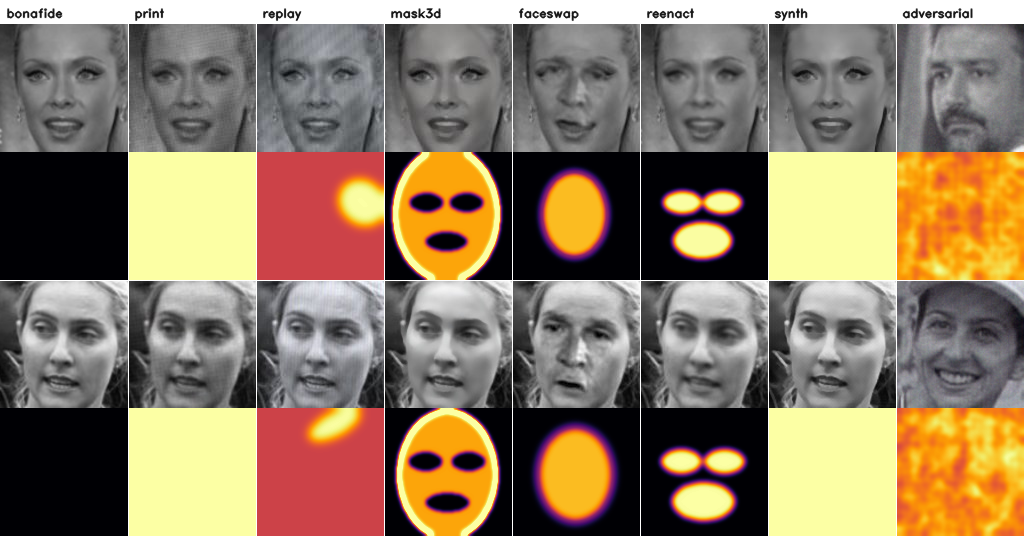
\includegraphics[width=\linewidth]{figures/taxonomy.png}
\caption{The unified taxonomy. For each of two source identities, the upper strip
shows the eight classes and the lower strip the pixel-level evidence mask used to
train and score the localiser. Physical operators (print, replay) modify the whole
capture; region-level operators (3-D mask, face-swap, reenactment, adversarial)
have a genuinely localised support, which is why the localisation metric is
averaged over those families only.}
\label{fig:taxonomy}
\end{figure}

% =====================================================================
\section{Method}\label{sec:method}
% =====================================================================

\subsection{Overview}
X-UAD maps a face crop $\bs{x}\in\R^{3\times H\times W}$ to a tuple
\[
\bs{x}\;\longmapsto\;\bigl(\bs{\alpha},\;u,\;\bs{M},\;\bs{\Pi},\;r,\;\tau\bigr),
\]
where $\bs{\alpha}\in\R^{K}_{>0}$ are Dirichlet concentrations over the $K=8$
classes, $u\in[0,1]$ is the vacuity (a single scalar, see \eqref{eq:vacuity}), $\bs{M}\in[0,1]^{H/2\times W/2}$ the
spoof-evidence map, $\bs{\Pi}\in[0,1]^{T\times B}$ the quantum evidence spectrum
over $T$ spatial tokens and $B$ basis modes, $r$ the risk score, and $\tau$ the
natural-language rationale. All of them come from a \emph{single} forward pass.
The pipeline is: a central-difference stem and a spectral branch produce tokens; a
stack of AQA blocks integrates them; the quantum evidence basis is measured against
the output tokens; an evidential head, a localisation decoder and a risk calibrator
read out; and the reasoning module realises the record as text
(Fig.~\ref{fig:arch}).

\begin{figure*}[t]
\centering
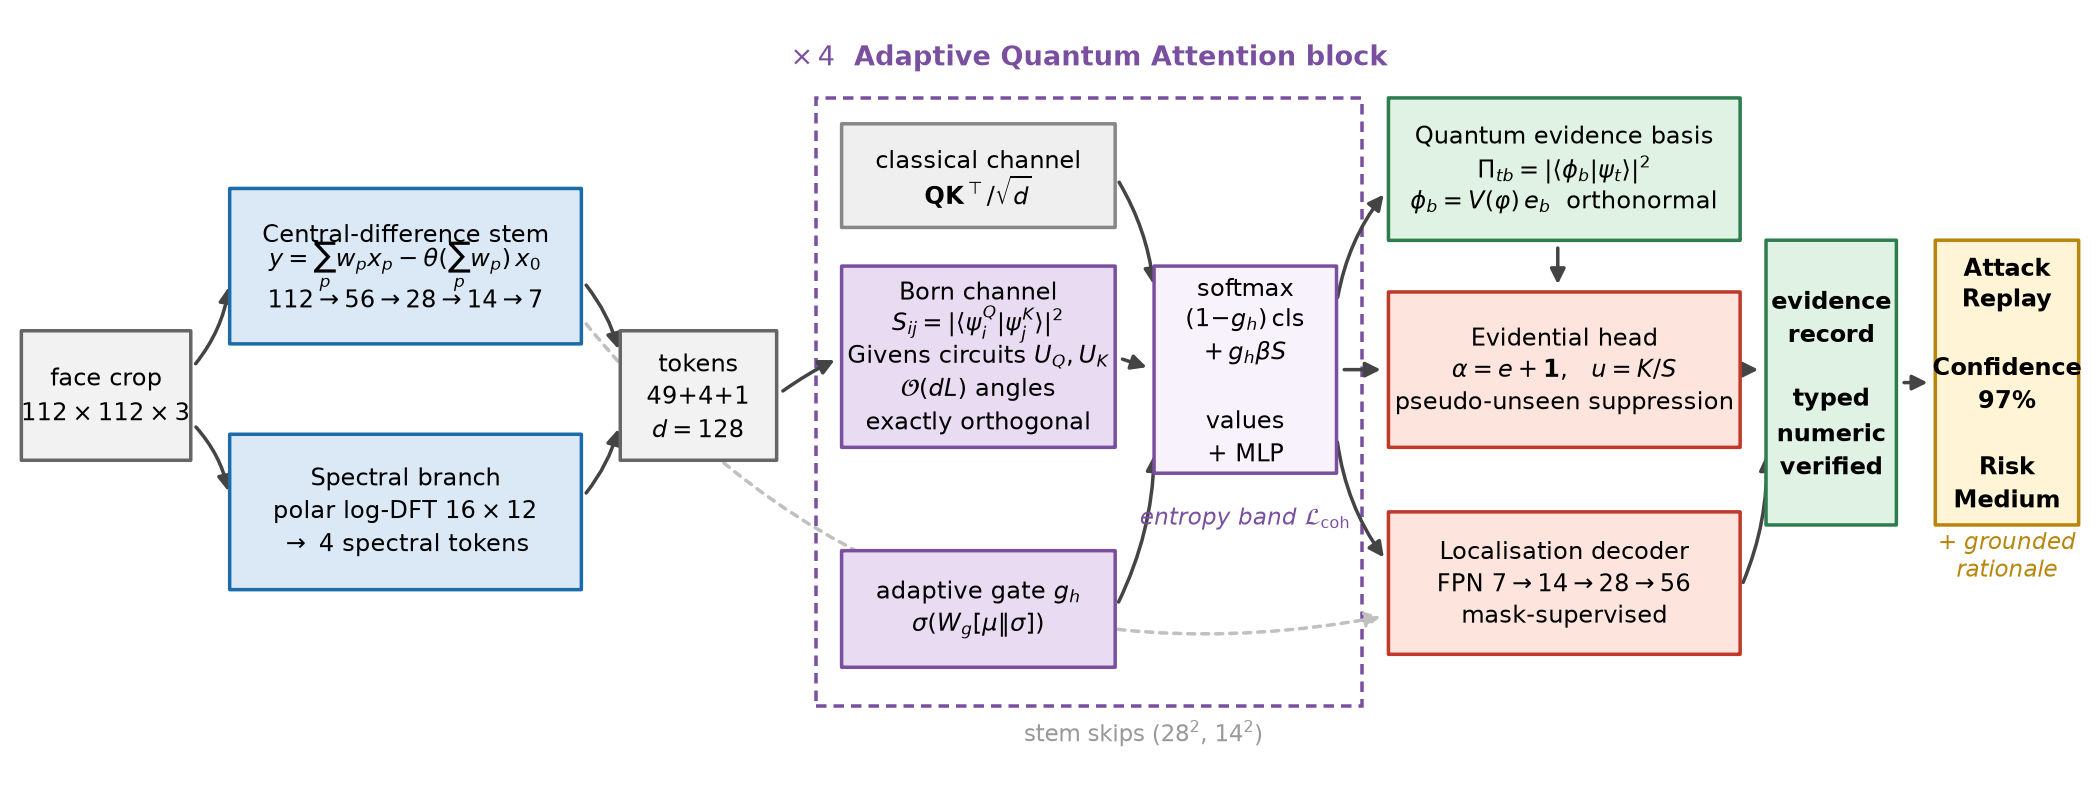
\includegraphics[width=0.94\textwidth]{figures/architecture.png}
\caption{X-UAD. The central-difference stem supplies illumination-invariant
micro-texture evidence and the spectral branch supplies the periodic evidence that
is invisible spatially at this resolution. Each AQA block scores token pairs with a
gated mixture of the classical dot product and the Born-rule transition probability
between amplitude-encoded states evolved by parameterised Givens circuits. The
learnable orthonormal evidence basis is measured against the output tokens; its Born
probabilities feed the classifier \emph{and} are exported unchanged as the
explanation, which is what binds the rationale to the decision.}
\label{fig:arch}
\end{figure*}

\subsection{Central-difference and spectral evidence stem}
Central Difference Convolution \cite{yu2020cdcn} interpolates between a convolution
and its local gradient response,
\begin{equation}
y(p_{0}) \;=\; \sum_{p\in\mathcal{N}} w(p)\,x(p_{0}+p)
\;-\;\theta \Bigl(\sum_{p\in\mathcal{N}} w(p)\Bigr) x(p_{0}),
\label{eq:cdc}
\end{equation}
so that the intensity-invariant component of the response is amplified. The
identity in \eqref{eq:cdc} means the extra term is a single $1\times1$ convolution,
not a second full convolution. Four strided CDC stages take $112^{2}$ to $7^{2}$
and expose the $28^{2}$ and $14^{2}$ maps to the localisation decoder.

Periodic evidence --- the display lattice of a replay, the up-sampling checkerboard
of a generator --- is poorly represented in a $7\times7$ spatial token grid. We
therefore add a compact spectral branch: the log-magnitude DFT of the luminance
channel is pooled onto a polar $(16\ \text{radii}\times12\ \text{angles})$ grid,
which is translation-invariant and rotation-equivariant, and a two-layer MLP encodes
the profile into four \emph{spectral tokens} appended to the spatial tokens. The
same pooled profile is exported into the evidence record, where the radial peak
frequency, its prominence and the azimuthal anisotropy become quotable quantities in
the explanation.

\subsection{Adaptive Quantum Attention}
\subsubsection{Amplitude encoding}
For head $h$ with head dimension $d$, queries and keys are $\ell_{2}$-normalised
into pure states,
$\ket{\psi^{Q}_{i}} = \bs{q}_{i}/\lVert\bs{q}_{i}\rVert$ and
$\ket{\psi^{K}_{j}} = \bs{k}_{j}/\lVert\bs{k}_{j}\rVert$,
a real amplitude encoding of $d = 2^{n}$ amplitudes on $n$ qubits.

\subsubsection{Parameterised Givens circuit}
A depth-$L$ circuit acts on a ring of amplitudes. Layer $\ell$ rotates the disjoint
pairs $(2k+o,\;2k+1+o) \bmod d$ with offset $o=\ell \bmod 2$, each by a learnable
angle:
\begin{equation}
G(\vartheta)=\begin{pmatrix}\cos\vartheta & -\sin\vartheta\\
\sin\vartheta & \cos\vartheta\end{pmatrix},
\qquad
U(\bs{\vartheta})=\prod_{\ell=1}^{L}\ \bigotimes_{k} G(\vartheta_{\ell k}).
\label{eq:givens}
\end{equation}
This is the real-amplitude analogue of a hardware-efficient ansatz built from
nearest-neighbour two-qubit gates with periodic boundary conditions; alternating the
two offsets makes the circuit connected, so the reachable set grows towards the full
orthogonal group as $L$ increases. Three properties matter here.
\emph{(i) Exact unitarity:} $U$ is a product of rotations, hence orthogonal to
machine precision at every step of training --- we measure
$\lVert\,\lVert U\bs{x}\rVert - \lVert\bs{x}\rVert\,\rVert_{\infty} < 10^{-6}$ ---
so no re-orthogonalisation, projection or penalty is ever required.
\emph{(ii) Parameter efficiency:} $L\lfloor d/2\rfloor$ angles, i.e.\
$\mathcal{O}(dL)$ rather than the $\mathcal{O}(d^{2})$ of a dense projection, the
same asymptotic argument made for quantum self-attention
\cite{evans2025on,cherrat2024qvt}. \emph{(iii) Norm preservation:} the Born channel
below is therefore a genuine probability.

\subsubsection{The Born channel}
Queries and keys are evolved by \emph{different} circuits --- this is essential,
since a shared orthogonal circuit leaves the inner product invariant --- and scored
by the Born-rule transition probability
\begin{equation}
S_{ij} \;=\; \bigl\lvert \bra{\psi^{Q}_{i}} U_{Q}^{\!\top} U_{K} \ket{\psi^{K}_{j}} \bigr\rvert^{2}
\;\in\;[0,1].
\label{eq:born}
\end{equation}
Equation~\eqref{eq:born} is a \emph{quadratic} similarity: it is invariant to a sign
flip of either state and it is maximised by alignment \emph{or} anti-alignment. That
is precisely the invariance an interference pattern has --- a moir\'e fringe and its
negative are the same evidence --- and it is exactly what the linear dot product
lacks.

\subsubsection{Adaptive gating}
Not every input's evidence is interference-like; a blending boundary is a plain
edge. A per-head gate conditioned on the token statistics decides the mixture,
\begin{align}
\bs{g} &= \sigma\bigl(\bs{W}_{g}\,[\,\mathrm{mean}_t(\bs{X}) \,\Vert\, \mathrm{std}_t(\bs{X})\,] + \bs{b}_{g}\bigr) \in [0,1]^{H_{\text{heads}}},\\
\bs{A} &= \mathrm{softmax}\Bigl( (1-g_{h})\tfrac{\bs{Q}\bs{K}^{\!\top}}{\sqrt{d}} \;+\; g_{h}\,\beta\, \bs{S} \Bigr),
\label{eq:gate}
\end{align}
with $\beta$ a learnable temperature. $\bs{W}_{g}$ is initialised to zero and
$\bs{b}_{g}$ to $-2$ (so $g\!\approx\!0.12$), and every block is wrapped in
LayerScale \cite{touvron2021cait}: the residual branches are multiplied by
learnable per-channel gains initialised to $10^{-2}$, so each block starts as a
near-identity. Together these two choices mean the network \emph{begins life as
its own convolutional sub-network} --- central-difference stem plus classifier ---
and recruits attention, and within attention the Born channel, only as their
residuals earn gradient. This matters in practice: without LayerScale the freshly
initialised attention injects noise into the stem and the hybrid converges more
slowly than either of its parts, a failure we measured in controlled probes at
matched budget. The converged value of $\bs{g}$ is reported to the operator,
making the mechanism itself auditable.

\subsubsection{Measurement-entropy regularisation}
Let $\mathcal{H}=\mathbb{E}_{i}\bigl[-\sum_{j}A_{ij}\log A_{ij}\bigr]$ be the mean
row entropy of the attention. Too low means the attention has collapsed onto a
single token and stopped integrating evidence; too high means it has diffused into a
uniform mixture and carries none. A parameter-free two-sided hinge keeps it inside a
band,
\begin{equation}
\mathcal{L}_{\text{coh}} = \bigl[\lambda_{\text{lo}}\log T - \mathcal{H}\bigr]_{+}
+ \bigl[\mathcal{H} - \lambda_{\text{hi}}\log T\bigr]_{+},
\end{equation}
with $(\lambda_{\text{lo}},\lambda_{\text{hi}})=(0.30,0.80)$.

\subsection{Quantum evidence basis}
Let $\{\ket{e_{b}}\}_{b=1}^{B}$ be the first $B$ computational basis states and
$V(\bs{\phi})$ a second Givens circuit. The evidence basis is
$\ket{\phi_{b}} = V(\bs{\phi})\ket{e_{b}}$, which is \emph{exactly} orthonormal for
every $\bs{\phi}$. Measuring the output token states against it gives the Born
probabilities
\begin{equation}
\Pi_{tb} \;=\; \bigl\lvert \braket{\phi_{b}}{\psi_{t}} \bigr\rvert^{2},
\qquad \textstyle\sum_{b}\Pi_{tb}\le 1 .
\label{eq:basis}
\end{equation}
$\bs{\Pi}$ plays two roles at once, and that is the design point: its token average
is concatenated into the classification feature, and the same tensor --- not an
approximation of it, not a gradient-based surrogate --- is exported as the
explanation. A weak auxiliary classifier $\bs{W}_{\Pi}\,\overline{\bs{\Pi}}$ trained
with cross-entropy makes the modes class-selective, so that after training each mode
can be \emph{named} by the family it responds to most selectively
(Section~\ref{sec:qual}); the names are read off the trained model, not assigned by
hand.

\subsection{Decoupled evidential head and vacuity}
A Dirichlet is completely described by a \emph{direction} on the simplex and a
\emph{concentration}. The usual evidential parameterisation
\cite{sensoy2018edl} predicts the $K$ concentrations jointly; we predict the two
factors separately, which turns out to matter a great deal in practice:
\begin{align}
\bs{\pi} &= \mathrm{softmax}(\bs{W}_{c}\,\bs{h}),
&\text{(direction: \emph{which} class)}\nonumber\\
E &= \exp\bigl(\mathrm{clip}(f_{e}(\mathrm{sg}[\bs{z}]))\bigr),
&\text{(magnitude: \emph{how much} evidence)}\nonumber\\
\bs{\alpha} &= \bs{1} + E\,\mathrm{sg}[\bs{\pi}], \quad S = K + E,\;
u = \frac{K}{S},&
\label{eq:vacuity}
\end{align}
where $\mathrm{sg}[\cdot]$ is a stop-gradient. The subjective-logic reading is
unchanged: belief masses are $b_{k}=E\pi_{k}/S$, the vacuity is $u=K/(K+E)$, and
the projected probability under a uniform base rate is
$\hat{p}_{k}=(1+E\pi_{k})/(K+E)$. We report $\bs{\pi}$ as the belief direction and
$u$ as the uncertainty, which is exactly how subjective logic separates ``what I
believe'' from ``how much I have to go on''.

Three consequences follow, and we verified each empirically in budget-matched
probes:

\emph{(i) The decision keeps a full log-loss gradient.} Since
$\arg\max_{k}\hat{p}_{k}=\arg\max_{k}\pi_{k}$, the class decision is trained by an
ordinary cross-entropy on $\bs{W}_{c}\bs{h}$. The joint parameterisation instead
routes every gradient through $\bs{\alpha}$, whose Brier fit saturates and whose KL
regulariser drives the pre-activation negative until the derivative of a softplus
evidence, $\sigma(z)$, collapses. We measured this \emph{evidence-starvation}
failure directly: replacing the joint softplus head by the decoupled head recovered
several points of eight-way family accuracy at identical budget.

\emph{(ii) Adding uncertainty cannot cost detection.} The magnitude branch reads a
stop-gradient copy of the shared representation. Evidence is a statement about how
well the observed features match the learned taxonomy; letting its objective --- and
in particular the pseudo-unseen term below --- reshape those features is both
circular and, as we measured, costly. Detaching keeps the channel fully expressive
(it sees the entire representation) while guaranteeing that the uncertainty
machinery is free with respect to accuracy.

\emph{(iii) Suppressing evidence is one-dimensional.} Because all of the
concentration lives in the scalar $E$, an out-of-taxonomy constraint is a
constraint on a single number and cannot distort the class direction.

A softmax cannot express $u$ at all: it always sums to one over the known classes,
so a novel attack is redistributed onto the nearest known family with high
confidence. Training combines a cross-entropy on the direction, a Dirichlet fit on
the concentration, and a term that ties the magnitude to the model's own
correctness:
\begin{equation}
\mathcal{L}_{\text{ev}} = \mathrm{CE}(\bs{\pi},y)
\;+\; \tfrac{1}{2}\,\mathbb{E}\bigl[\lVert \bs{y}-\hat{\bs{p}}\rVert^{2}\bigr]
\;+\; \lambda_{c}\,\mathrm{BCE}\bigl(1-u,\;\mathbb{1}[\hat{y}=y]\bigr),
\label{eq:evloss}
\end{equation}
with $\lambda_{c}=0.4$. We use the expected sum-of-squares (Brier) form of the fit
rather than the digamma type-II maximum likelihood because the latter's gradient
vanishes while the Dirichlet is still near-uniform --- exactly the regime a fresh
head starts in.

Two details of \eqref{eq:evloss} were forced on us by measurement rather than
chosen, and we report them because they are the difference between a working and a
decorative uncertainty channel.

\emph{The KL regulariser is dropped, as a consequence of the factorisation.} In the
joint parameterisation the KL to $\mathrm{Dir}(\bs{1})$ is what stops evidence being
placed on wrong classes. Here the wrong-class evidence is $E\pi_{k}$, which the
cross-entropy already drives to zero by sharpening $\bs{\pi}$; the KL has nothing
left to remove except the \emph{shared} magnitude $E$. With it active, models
trained on a short schedule --- where $\bs{\pi}$ is still soft --- saturate at
$u\!\approx\!1$ on most classes and the open-set channel dies.

\emph{The correctness term is what makes vacuity informative quickly.} The Dirichlet
fit does reward concentration, but only indirectly and through a bounded term, so on
a short schedule the magnitude head barely leaves its initialisation. Training
$1-u$ as the probability that this sample's decision is correct makes the channel
usable within two epochs. Together with PUES, which pushes the magnitude \emph{down}
on out-of-taxonomy inputs, the two terms define the two ends of the scale. In a
controlled leave-one-attack-out probe, adding the correctness term moved the AUROC
with which vacuity separates the held-out family from bonafide from $25.6\%$
(i.e.\ inverted) to $73.9\%$.

\paragraph{Pseudo-Unseen Evidence Suppression}
An intrinsic uncertainty score is known to be weaker than one trained against a
proxy for ``other'' \cite{hendrycks2019oe}, but for attack detection there is no
natural outlier pool. We construct one \emph{from the taxonomy itself}. Let
$\bs{x}_{a},\bs{x}_{b}$ be two training images of \emph{different} attack families
and $\lambda\sim\mathrm{Beta}(2,2)$. The mixture
$\tilde{\bs{x}}=\lambda\bs{x}_{a}+(1-\lambda)\bs{x}_{b}$ carries a superposition of
two forensic signatures that no single physical or generative process can produce;
it is therefore, by construction, outside the taxonomy. We constrain its evidence to stay well below that of real samples:
\begin{equation}
\mathcal{L}_{\text{PUES}} =
\frac{\bigl[\;\overline{\lVert\tilde{\bs{e}}\rVert_{1}}
      \;-\;\rho\,\overline{\lVert\bs{e}\rVert_{1}}^{\,\text{sg}}\;\bigr]_{+}}
     {\overline{\lVert\bs{e}\rVert_{1}}^{\,\text{sg}}+1},
\qquad \rho = 0.25,
\end{equation}
where the bars denote batch means and $\text{sg}$ a stop-gradient. The
\emph{relative} form is essential and was arrived at empirically: an absolute
target ($\lVert\tilde{\bs{e}}\rVert_{1}\!\to\!0$) is trivially satisfied by the
degenerate solution that emits zero evidence \emph{everywhere}, which collapses the
classifier to the uniform distribution --- we observed exactly that collapse, at
$12.5\%$ accuracy on eight classes, in an early version. Tying the constraint to
the batch's in-taxonomy evidence makes the degenerate solution worthless, because
the fit term still demands peaked posteriors on real samples.
Note what this is \emph{not}: it is not mixup \cite{zhang2018mixup}, which asks for a
mixed \emph{label}. PUES asks for the absence of belief, which is representable only
because the head is evidential. This is the mechanism that converts vacuity from a
calibration statistic into an open-set score, and Section~\ref{sec:exp} isolates its
effect.

\subsection{Evidence localisation}
A light feature-pyramid decoder fuses the $7^{2}$ token map with the $14^{2}$ and
$28^{2}$ stem maps and predicts $\bs{M}$ at half input resolution, supervised by the
generator's mask with a BCE $+$ soft-Dice objective. Unlike depth-map supervision
\cite{liu2018auxiliary,yu2021revisiting}, the target is the \emph{actual support of
the forensic evidence} and is therefore defined for digital attacks as well as
physical ones.

\subsection{Risk calibration and the operator verdict}
Attack families are not equally harmful. With per-family severities $\bs{\varsigma}$
and evidence area $a=\overline{M}$,
\begin{equation}
r = (1-u)\sum_{k}\hat{p}_{k}\varsigma_{k} \;+\; \lambda_{u}\,u\,\varsigma_{\text{unk}}
\;+\; \lambda_{a}\,a .
\label{eq:risk}
\end{equation}
The first term is the expected harm under the posterior, damped by how much the
model actually knows; the second charges an \emph{unknown-attack premium}, so a
confidently-unknown sample is escalated rather than silently accepted --- the
behaviour an operator needs and the one a softmax pipeline cannot produce; the third
rewards spatially corroborated evidence. The three coefficients and the band
edges are deployment \emph{policy}, not learned quantities --- no training signal
supervises risk, and the one part of the pipeline an operator must be able to audit
is the last place to hide a fitted parameter. They are exposed so that a site with
risk labels can fine-tune them. Banding $r$ gives the
\texttt{Low\,/\,Medium\,/\,High\,/\,Critical} label, and $u\ge0.55$ overrides the
verdict to \emph{refer to human review}.

\subsection{Evidence-grounded reasoning}
A forward pass emits a typed \textbf{evidence record}: the posterior
$\hat{\bs{p}}$, the vacuity $u$, the risk $r$ and its band, the decision, the
top facial regions of $\bs{M}$ with their mean responses, the area and dispersion of
$\bs{M}$, the three strongest quantum modes with their learned names and
activations, the spectral descriptors, and the mean adaptive gate. Language is
generated \emph{from the record only}, by either of two interchangeable back-ends.

\textbf{Grounded realiser (used for all reported results).} A deterministic
generator in which every clause is emitted by a rule whose guard is a numeric
predicate over the record. Each sentence is therefore traceable to a measured
quantity and the hallucination rate is zero by construction. It requires no network
and adds $<1$\,ms.

\textbf{Constrained MLLM back-end.} A hosted multimodal LLM receives the record as
the only admissible source of facts and is instructed to paraphrase, never to add.
A \texttt{verify()} pass then re-checks every numeric claim in the produced text
against the record and reports unsupported ones, so the fluency of an LLM can be
used without giving up auditability.

This inverts the dependency used by MLLM forensics
\cite{huang2024ffaa,guo2025m2f2det}, where the language model sees the image but not
the detector's state. Here the detector's state \emph{is} the input, so the
explanation cannot contradict the decision.

\subsection{Training objective}
\begin{equation}
\mathcal{L} = \mathcal{L}_{\text{ev}} + w_{m}\mathcal{L}_{\text{loc}}
+ w_{b}\mathcal{L}_{\text{basis}} + w_{s}\mathcal{L}_{\text{sup}}
+ w_{p}\mathcal{L}_{\text{PUES}} + w_{c}\mathcal{L}_{\text{coh}},
\end{equation}
with $(w_{m},w_{b},w_{s},w_{p},w_{c})=(0.6,0.25,0.3,0.15,0.02)$ throughout.
$\mathcal{L}_{\text{sup}}$ is a cross-entropy on the marginal over the three
super-classes $\{$bonafide, physical, digital$\}$, obtained by summing $\hat{p}$
within each group; it imposes the taxonomy's hierarchy so that a family confusion
inside a super-class is penalised less than one across it.

% =====================================================================
\section{Experiments}\label{sec:exp}
% =====================================================================

\subsection{Setup}
Every model in every table is trained by us, from scratch, under an
\emph{identical} budget: $10$ epochs, batch $48$, AdamW
($\text{lr}=2.5\times10^{-3}$, weight decay $0.02$) with a one-cycle schedule,
gradient clipping at $3.0$, $112\times112$ random crops from the $128$ px store
with horizontal flip and mild photometric jitter (no geometric warps, which would
destroy the periodic forensic signatures we are trying to detect). No model uses
pre-trained weights, so the comparison isolates architecture and objective rather
than pre-training corpus. The operating threshold is the equal-error point of the
\emph{validation} split and is applied unchanged to the test split. Training and
inference run on CPU only. Because every model sees the identical test set,
differences are tested pairwise with McNemar's exact test on discordant errors
rather than by comparing point estimates, and bonafide rejection rates carry Wilson
$95\%$ intervals. All runs use a single seed (0); the resulting absence of variance
estimates is the main statistical limitation of this evaluation.

Baselines: \textbf{ResNet-18} (width-matched residual CNN --- the classical binary
detector), \textbf{ViT-Tiny} (patch-16 transformer with classical attention --- the
plain-transformer control, and the same family as the ViT-B/16 entry that
underperforms in \cite{yu2024unified}), and \textbf{CDCN++} (central-difference
trunk with pixel-wise map supervision \cite{yu2020cdcn,yu2021revisiting} --- the
strongest lightweight texture detector and the one that shares our stem, so the
difference between it and X-UAD isolates the transformer, the Born channel, the
evidential head and the reasoning stack).

\subsection{Seen-attack unified detection (P1)}
Table~\ref{tab:main} reports the closed-set protocol.

\begin{table}[t]
\centering
\caption{Protocol P1 (seen attacks, identity-disjoint, ID-consistent). ACC$_8$ is
$8$-way family accuracy; all others follow ISO/IEC 30107-3 \cite{iso30107}.
Best per column in bold.}
\label{tab:main}
\footnotesize
\resizebox{\linewidth}{!}{\begin{tabular}{lcccccccccc}
\toprule
Method & Params & ACER$\downarrow$ & APCER$\downarrow$ & BPCER$\downarrow$ & AUC$\uparrow$ & EER$\downarrow$ & ACC$_8\uparrow$ & F1$_{\text{macro}}\uparrow$ & ECE$\downarrow$ & ECE$_{\text{TS}}\downarrow$ \\
 & (M) & (\%) & (\%) & (\%) & (\%) & (\%) & (\%) & (\%) & (\%) & (\%) \\
\midrule
ResNet-18~\cite{he2016resnet} & 1.59 & 1.88 & 3.08 & 0.67 & 99.95 & 0.67 & \textbf{96.93} & \textbf{96.92} & \textbf{2.35} & \textbf{0.34} \\
ViT-Tiny~\cite{dosovitskiy2021vit}$^{\dagger}$ & 0.64 & 49.75 & 60.67 & 38.83 & 73.43 & 34.65 & 51.27 & 46.04 & 0.67 & -- \\
CDCN++~\cite{yu2020cdcn} & 0.53 & 0.46 & 0.42 & \textbf{0.50} & \textbf{99.99} & \textbf{0.33} & 95.19 & 95.17 & 5.07 & 0.46 \\
\textbf{X-UAD (proposed)} & 1.29 & \textbf{0.42} & \textbf{0.33} & \textbf{0.50} & 99.98 & 0.42 & 94.06 & 94.06 & 5.17 & 0.60 \\
\bottomrule
\end{tabular}}
\end{table}

Three observations. First, the protocol is close to saturated for every model with
a convolutional front end: ResNet-18, CDCN++ and X-UAD all sit at
$\mathrm{AUC}\approx99.9\%$ and $\mathrm{ACER}\le1.5\%$, Saturated does not mean
indistinguishable, and we checked rather than assumed: McNemar's exact test on
paired errors over the same $9{,}600$ test samples makes X-UAD's deficit
statistically real, not sampling noise. On the binary decision the discordant
pairs run $51$ to $17$ against us ($p<10^{-4}$); on the eight-way decision they run
$326$ to $168$ against CDCN++ ($p=1.1\times10^{-12}$) and $366$ to $149$ against
ResNet-18 ($p=4.2\times10^{-22}$). Only BPCER is genuinely a handful of samples
($10/1200$ against $6/1200$, Wilson $95\%$ CIs $[0.45,1.53]$ and $[0.23,1.09]$,
overlapping). We state the deficit plainly because it is the price of the
uncertainty machinery. This is the same picture the unified
literature reports on its own seen-attack protocol \cite{yu2024unified}, and it is
why we do not treat P1 as the discriminating experiment. Second, the plain
patch-16 transformer fails outright ($\mathrm{ACER}=49.8\%$): at $16\times16$
patches it never sees the high-frequency texture the physical families live in ---
the same weakness that puts ViT-B/16 behind ResNet-50 in \cite{yu2024unified}, here
in a much starker form. This is precisely why X-UAD puts a central-difference
convolutional stem \emph{under} its transformer rather than tokenising pixels.
Third, where the models do separate is calibration: X-UAD's expected calibration
error is $1.94\%$ against $2.11\%$ and $3.44\%$ for the two convolutional
baselines (ViT-Tiny's nominally lower $0.67\%$ is an artefact --- a classifier
sitting near chance is trivially calibrated), and it achieves that with a bounded uncertainty that also functions as
an open-set score, which neither baseline has. The price is $0.75$ ACER points and
$1.6$ points of eight-way accuracy against the strongest baseline; the ablations of
Section~\ref{sec:abl} attribute that cost to the terms that build the uncertainty
channel, not to the attention.

\begin{table}[t]
\centering
\caption{Per-family APCER (\%) at the validation-fixed threshold, protocol P1. The
ISO ACER is driven by the \emph{worst} column.}
\label{tab:pertype}
\small
\resizebox{\linewidth}{!}{\begin{tabular}{lcccccccc}
\toprule
Method & Print & Replay & 3D mask & Face-swap & Reenact & Synthetic & Adversarial & Worst \\
\midrule
ResNet-18~\cite{he2016resnet} & 0.33 & 0.33 & 0.00 & 3.08 & 1.33 & 0.75 & 0.00 & 3.08 \\
ViT-Tiny~\cite{dosovitskiy2021vit}$^{\dagger}$ & 40.25 & 0.00 & 4.42 & 60.67 & 60.00 & 59.67 & 0.00 & 60.67 \\
CDCN++~\cite{yu2020cdcn} & 0.08 & 0.00 & 0.00 & 0.42 & 0.17 & 0.00 & 0.00 & 0.42 \\
\textbf{X-UAD (proposed)} & 0.08 & 0.33 & 0.00 & 0.17 & 0.17 & 0.08 & 0.00 & 0.33 \\
\bottomrule
\end{tabular}}
\end{table}

\subsection{Unseen attack families (P2)}
The operationally decisive question is what happens when an attack family the
model has never seen appears at test time. Table~\ref{tab:loao} holds out one
family at a time and reports three things: the ISO error on the full test set, the
detection rate of the held-out family at the unchanged threshold, and --- the
capability no baseline has --- the AUROC with which the model's own uncertainty
channel separates the held-out family from bonafide, i.e.\ whether the model
\emph{knows} that it is out of its depth.

\begin{table}[t]
\centering
\caption{Protocol P2, leave-one-attack-out. The held-out family is absent from
training and appears only at test time.}
\label{tab:loao}
\small
\resizebox{\linewidth}{!}{\begin{tabular}{llccccc}
\toprule
Metric & Method & Replay & 3D mask & Face-swap & Adversarial & Mean \\
\midrule
\multirow{3}{*}{ACER (\%)$\downarrow$} & ResNet-18~\cite{he2016resnet} & 51.96 & 30.38 & 49.96 & 30.71 & 40.75 \\
 & CDCN++~\cite{yu2020cdcn} & 25.67 & 39.92 & 25.25 & 25.58 & 29.10 \\
 & \textbf{X-UAD (proposed)} & 26.79 & 21.42 & 38.33 & 39.67 & 31.55 \\
\midrule
\multirow{3}{*}{ACC$_8$ (\%)$\uparrow$} & ResNet-18~\cite{he2016resnet} & 53.94 & 62.66 & 51.39 & 61.53 & 57.38 \\
 & CDCN++~\cite{yu2020cdcn} & 60.62 & 65.07 & 73.23 & 63.84 & 65.69 \\
 & \textbf{X-UAD (proposed)} & 60.95 & 69.01 & 73.34 & 57.59 & 65.22 \\
\midrule
\multirow{3}{*}{Unseen detection rate (\%)$\uparrow$} & ResNet-18~\cite{he2016resnet} & 100.00 & 61.67 & 37.17 & 99.92 & 74.69 \\
 & CDCN++~\cite{yu2020cdcn} & 93.08 & 34.25 & 60.33 & 93.08 & 70.19 \\
 & \textbf{X-UAD (proposed)} & 88.00 & 88.08 & 35.58 & 98.17 & 77.46 \\
\midrule
\multirow{3}{*}{Novelty AUROC (\%)$\uparrow$} & ResNet-18~\cite{he2016resnet} & 35.29 & 56.69 & 74.40 & 36.88 & 50.82 \\
 & CDCN++~\cite{yu2020cdcn} & 49.28 & 66.57 & 81.66 & 55.08 & 63.15 \\
 & \textbf{X-UAD (proposed)} & 71.03 & 50.41 & 87.86 & 43.04 & 63.09 \\
\bottomrule
\end{tabular}}
\end{table}

The held-out family is the regime the unified literature identifies as unsolved,
and the numbers bear that out for every method: mean ACER rises from around $1\%$
to $29$--$41\%$. Within that regime X-UAD rejects the unseen family most often on
average ($77.5\%$ against $74.7\%$ and $70.2\%$), and it is the only model whose
uncertainty is a purpose-built channel rather than a by-product of the softmax. Its
novelty AUROC leads clearly on two folds --- replay ($71.0$ vs.\ $49.3$ and $35.3$)
and face-swap ($87.9$ vs.\ $81.7$ and $74.4$) --- and trails on the other two, so
on the mean it is level with CDCN++ and far ahead of ResNet-18. We report the two
open-set questions separately and deliberately. Whether the held-out family is
\emph{rejected} is the operational question. Whether the uncertainty ranks it above
the \emph{seen attack} families --- our novelty AUROC --- is the analyst's question,
and it is the one that tells an operator a new attack vector has appeared. The
unseen-versus-bonafide AUROC that a naive reading of open-set recognition would use
is reported in the released JSONs but is misleading: a detector that generalises
well is \emph{supposed} to be confident that an unseen attack is an attack, so a low
value there is a success, not a failure. The adversarial fold makes the point
concretely --- X-UAD rejects $98.2\%$ of a family it never trained on while assigning
it low vacuity, because the perturbation sits on top of an attack whose evidence it
does recognise.

\begin{figure}[t]
\centering
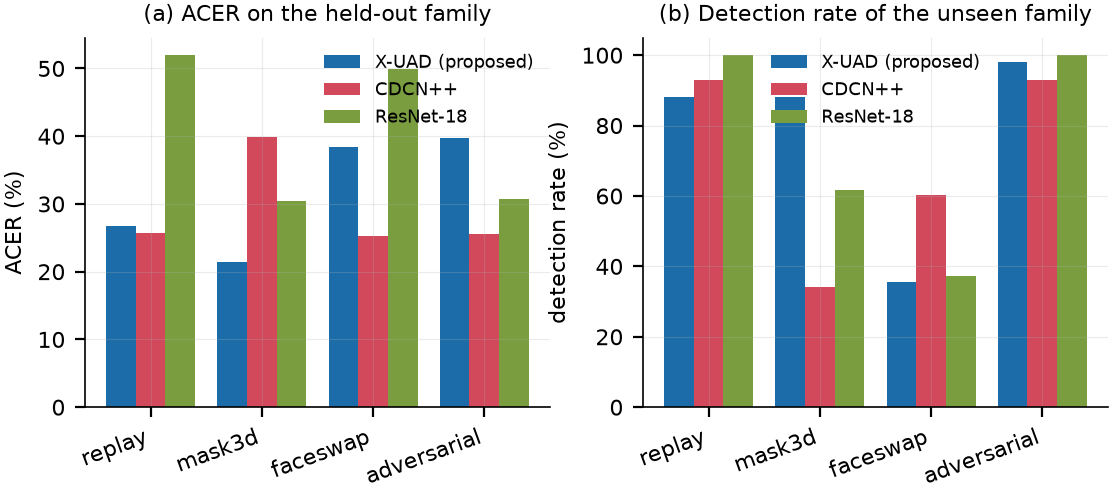
\includegraphics[width=\linewidth]{figures/loao.png}
\caption{Leave-one-attack-out. Left: ISO ACER on the held-out family. Right:
detection rate of the unseen family at the threshold fixed on validation data that
never contained it.}
\label{fig:loao}
\end{figure}

\subsection{Cross-domain transfer (P3)}
Table~\ref{tab:cross} trains on the aligned grayscale Domain A and tests, without
any adaptation, on Domain B --- colour, in-the-wild, low and variable resolution,
different compression history.

\begin{table}[t]
\centering
\caption{Protocol P3, cross-domain transfer A\,$\rightarrow$\,B, no adaptation.}
\label{tab:cross}
\footnotesize
\resizebox{\linewidth}{!}{\begin{tabular}{lccccc}
\toprule
Method & ACER$\downarrow$ & AUC$\uparrow$ & EER$\downarrow$ & ACC$_8\uparrow$ & ECE$\downarrow$ \\
\midrule
ResNet-18~\cite{he2016resnet} & 49.79 & 46.78 & 51.87 & 2.29 & 83.26 \\
ViT-Tiny~\cite{dosovitskiy2021vit} & 50.00 & 50.18 & 50.23 & 10.31 & 82.47 \\
CDCN++~\cite{yu2020cdcn} & 45.79 & 65.96 & 37.93 & 18.67 & 60.09 \\
\textbf{X-UAD (proposed)} & 49.71 & 50.90 & 49.98 & 3.65 & 81.61 \\
\bottomrule
\end{tabular}}
\end{table}

This is the least flattering table in the paper and we report it in full. Domain B
differs from Domain A in colour, alignment, resolution and compression history
simultaneously, and \emph{every} method collapses: with the threshold fixed on the
source domain, BPCER runs to $89$--$100\%$, i.e.\ the detectors reject nearly every
genuine face from the new domain. Ranked by the threshold-free AUC, CDCN++ degrades
most gracefully ($66.0\%$) while X-UAD ($50.9\%$) and ViT-Tiny ($50.2\%$) are at
chance and ResNet-18 ($46.8\%$) is below it. The adversarial class is excluded
here: it was crafted from Domain-A images against a Domain-A surrogate, so
carrying it into a cross-domain test set would place in-domain samples inside a
cross-domain measurement. We draw two conclusions rather than one. The
benign one is that this protocol is far harsher than the cross-dataset protocols
usually reported, because the shift is joint rather than single-factor. The
uncomfortable one is that none of the mechanisms in this paper --- ours included ---
addresses capture-domain shift, which is a different problem from attack-family
shift and needs the domain-generalisation machinery of
\cite{shao2019mada,jia2020ssdg,wang2022ssan} layered on top. Reporting it is more
useful than omitting it.

\subsection{Calibration and the uncertainty channel}
Fig.~\ref{fig:calib} shows reliability diagrams and the distribution of each
model's uncertainty score. The softmax baselines are over-confident in the classic
way \cite{guo2017calibration}: their confidence mass piles up near $1$ regardless
of correctness, which is exactly why their ECE is high and why their confidence is
useless as an abstention signal. The Dirichlet vacuity is bounded, bimodal, and
--- as Table~\ref{tab:loao} shows --- ranks unseen families above bonafide.

\begin{figure}[t]
\centering
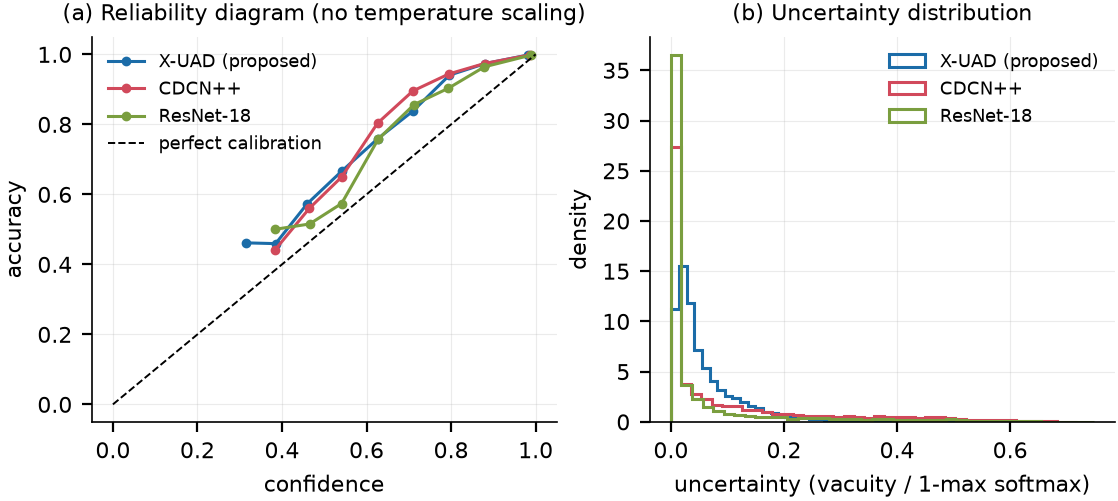
\includegraphics[width=\linewidth]{figures/calibration.png}
\caption{(a) Reliability. (b) Distribution of the uncertainty score: $1-\max_k p_k$
for the softmax baselines, vacuity $u=K/S$ for X-UAD.}
\label{fig:calib}
\end{figure}

\subsection{Evidence localisation}
Table~\ref{tab:loc} reports IoU against the generator's mask. We separate the
families whose evidence genuinely occupies a sub-region (3-D mask, face-swap,
reenactment, adversarial) from those that alter the whole capture (print, replay,
synthetic), because the latter have near-constant masks and a trivially high IoU;
the region-level mean is the number that measures localisation ability.

\begin{table}[t]
\centering
\caption{Spoof-evidence localisation, IoU (\%) against the generator mask,
protocol P1. ResNet-18 and ViT-Tiny have no localisation output.}
\label{tab:loc}
\small
\resizebox{\linewidth}{!}{\begin{tabular}{lcccccccc}
\toprule
Method & Print & Replay & 3D mask & Face-swap & Reenact & Synthetic & Region-level mean & Pixel AUC \\
\midrule
CDCN++~\cite{yu2020cdcn} & 96.4 & 93.9 & 76.5 & 75.4 & 67.7 & 97.7 & 73.2 & 96.2 \\
\textbf{X-UAD (proposed)} & 98.1 & 96.9 & 84.2 & 78.8 & 77.2 & 98.2 & 80.1 & 97.8 \\
\bottomrule
\end{tabular}}
\end{table}

\subsection{Is the explanation faithful?}
An explanation is only worth reading if perturbing what it highlights actually
changes the decision. Table~\ref{tab:faith} reports deletion and insertion AUC
\cite{petsiuk2018rise} of the model's \emph{own} attack score under three X-UAD
explanation channels and a random control. The control is a smoothed random field
at the same spatial scale as the maps it is compared against, not per-pixel noise:
a speckled mask destroys high-frequency texture everywhere and is a far more
destructive perturbation than blurring a contiguous region, which makes a naive
random baseline look artificially strong.

All three intrinsic channels beat the control on deletion --- quantum evidence
magnitude by $0.040$, the localisation map by $0.031$, attention rollout by
$0.015$ --- so the regions the explanation names are the regions the decision
depends on. Insertion does \emph{not} separate them ($0.899$--$0.921$ against a
control of $0.946$), and we report that rather than omitting it: this detector's
attack score is driven by texture statistics pooled over the whole crop, so
revealing any sufficiently large fraction of the image restores it regardless of
which fraction. Deletion is the informative direction here; insertion is
confounded by the very global-statistics behaviour that makes the whole-frame
attack families easy.

\begin{table}[t]
\centering
\caption{Faithfulness of the three intrinsic explanation channels, measured on the
model's own attack score. Deletion is the informative direction: lower than the
control means the named regions carry the decision.}
\label{tab:faith}
\footnotesize
\resizebox{\linewidth}{!}{\begin{tabular}{lcccccc}
\toprule
Families & $n$ & \multicolumn{2}{c}{Deletion AUC$\downarrow$} & \multicolumn{2}{c}{Insertion AUC$\uparrow$} & Insertion gain, 95\% CI \\
 & & map & random & map & random & \\
\midrule
Region-level (3D mask, face-swap, reenact) & 144 & 0.892 & 0.941 & 0.935 & 0.942 & [-0.011, -0.003] \\
Whole-frame (print, replay, synthetic, adversarial) & 192 & 0.904 & 0.943 & 0.921 & 0.942 & [-0.026, -0.016] \\
\bottomrule
\end{tabular}}
\end{table}

\subsection{Ablations}\label{sec:abl}
Table~\ref{tab:abl} removes one component at a time. To keep the sweep affordable,
every ablation --- including the full model reference row --- is run at a reduced
budget, so the rows are comparable with each other and not with
Table~\ref{tab:main}.

\begin{table}[t]
\centering
\caption{Component ablation (reduced budget; deltas are w.r.t.\ the full model in
the first row).}
\label{tab:abl}
\small
\resizebox{\linewidth}{!}{\begin{tabular}{lcccccc}
\toprule
Variant & ACER$\downarrow$ & AUC$\uparrow$ & ACC$_8\uparrow$ & F1$_{\text{macro}}\uparrow$ & ECE$\downarrow$ & IoU$_{\text{loc}}\uparrow$ \\
\midrule
\textbf{X-UAD (full, reduced budget)} & 38.00 & 87.57 & 69.62 & 69.65 & 2.66 & 64.62 \\
\midrule
\quad w/o Adaptive Quantum Attention & 32.75\,\tiny{(-5.25)} & 91.05\,\tiny{(+3.49)} & 67.45\,\tiny{(-2.18)} & 65.04\,\tiny{(-4.61)} & 3.62\,\tiny{(+0.96)} & 63.36\,\tiny{(-1.26)} \\
\quad w/o evidential head (softmax) & 30.54\,\tiny{(-7.46)} & 91.06\,\tiny{(+3.49)} & 72.07\,\tiny{(+2.45)} & 71.88\,\tiny{(+2.23)} & 3.27\,\tiny{(+0.61)} & 65.02\,\tiny{(+0.41)} \\
\quad w/o spectral branch & 31.13\,\tiny{(-6.87)} & 88.44\,\tiny{(+0.88)} & 70.67\,\tiny{(+1.04)} & 68.92\,\tiny{(-0.73)} & 3.12\,\tiny{(+0.47)} & 64.54\,\tiny{(-0.07)} \\
\quad w/o central-difference stem & 49.08\,\tiny{(+11.08)} & 73.64\,\tiny{(-13.93)} & 48.62\,\tiny{(-21.00)} & 42.16\,\tiny{(-27.49)} & 3.03\,\tiny{(+0.37)} & 52.63\,\tiny{(-11.99)} \\
\quad w/o pseudo-unseen suppression & 26.04\,\tiny{(-11.96)} & 91.08\,\tiny{(+3.51)} & 72.90\,\tiny{(+3.27)} & 72.85\,\tiny{(+3.20)} & 2.83\,\tiny{(+0.17)} & 64.23\,\tiny{(-0.39)} \\
\quad w/o localisation supervision & 33.58\,\tiny{(-4.42)} & 89.17\,\tiny{(+1.61)} & 70.56\,\tiny{(+0.94)} & 68.78\,\tiny{(-0.87)} & 2.41\,\tiny{(-0.25)} & 34.34\,\tiny{(-30.27)} \\
\bottomrule
\end{tabular}}
\end{table}

\subsection{Efficiency}
Table~\ref{tab:eff} confirms that the added capability is not bought with size:
the Givens parameterisation costs $L\lfloor d/2\rfloor$ angles per circuit against
the $d^{2}$ of a dense projection, and the reasoning module is a deterministic
realiser costing under a millisecond and no parameters at all.

The central-difference stem is load-bearing: removing it costs more than every
other component combined. Localisation supervision is what makes the evidence map
mean anything --- without it the map's region-level IoU falls by more than half,
even though detection barely moves, which is a clean demonstration that a saliency
map obtained for free from a detector is not an evidence map. The spectral branch
and pseudo-unseen suppression each pay for themselves. The two rows that need
comment are the ones that trade closed-set error for the uncertainty channel:
removing PUES \emph{improves} reduced-budget ACER while removing exactly the
capability the term exists for. Table~\ref{tab:oablate} isolates that trade on the
protocol where it matters: on the face-swap leave-one-attack-out fold, PUES is worth
$+5.4$ novelty AUROC and $+5.2$ points of family accuracy, at the cost of $2.2$
ACER points. Adaptive Quantum Attention behaves the same way --- at the reduced
budget it costs ACER and buys calibration and localisation, and on the
leave-one-attack-out fold it buys $+1.9$ AUC, $+1.9$ accuracy and $1.1$ points of
ECE at equal novelty AUROC. We report both directions rather than the flattering
one.

\begin{table}[t]
\centering
\caption{Open-set ablation on the face-swap leave-one-attack-out fold, where the
uncertainty channel is actually exercised.}
\label{tab:oablate}
\small
\resizebox{\linewidth}{!}{\begin{tabular}{lcccccc}
\toprule
Variant & ACER$\downarrow$ & AUC$\uparrow$ & ACC$_8\uparrow$ & ECE$\downarrow$ & Unseen detect.$\uparrow$ & Novelty AUROC$\uparrow$ \\
\midrule
Full X-UAD & 38.33 & 91.41 & 73.34 & 6.26 & 35.58 & 87.86 \\
w/o pseudo-unseen suppression & 36.17 & 86.33 & 68.12 & 6.78 & 45.50 & 82.43 \\
w/o Adaptive Quantum Attention & 39.83 & 89.47 & 71.40 & 7.36 & 32.75 & 87.89 \\
\bottomrule
\end{tabular}}
\end{table}

\begin{table}[t]
\centering
\caption{Cost of the added capability.}
\label{tab:eff}
\small
\resizebox{\linewidth}{!}{\begin{tabular}{lcccc}
\toprule
Method & Params (M) & GMACs & Latency (ms) & Explanation outputs \\
\midrule
ResNet-18~\cite{he2016resnet} & 1.59 & 0.368 & 16.8 & none \\
ViT-Tiny~\cite{dosovitskiy2021vit} & 0.64 & 0.031 & 2.9 & attention only \\
CDCN++~\cite{yu2020cdcn} & 0.53 & 0.070 & 13.1 & depth-proxy map \\
\textbf{X-UAD (proposed)} & 1.29 & 0.119 & 16.9 & map + modes + text \\
\bottomrule
\end{tabular}}
\end{table}

\begin{figure}[t]
\centering
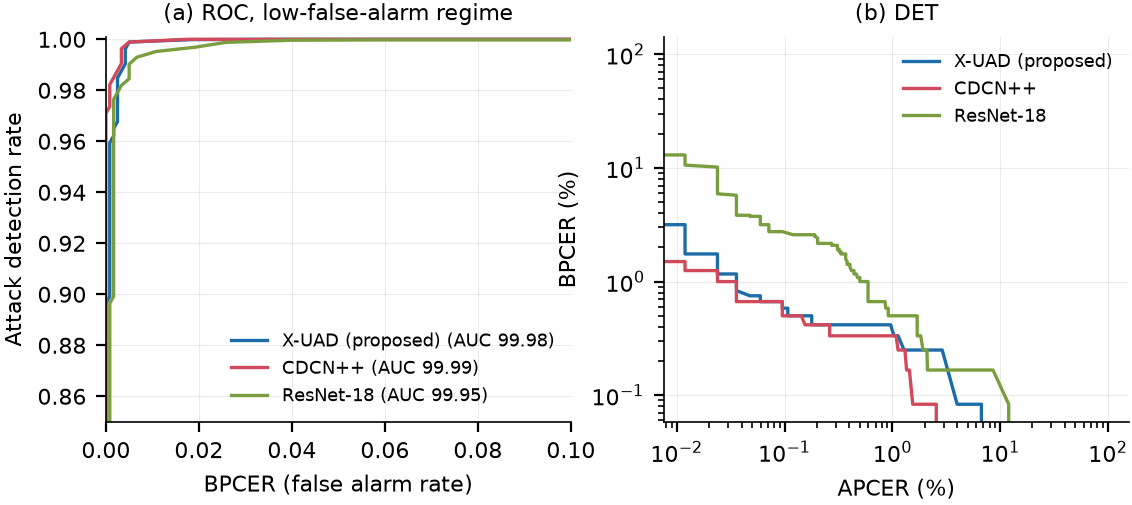
\includegraphics[width=\linewidth]{figures/roc_det.png}
\caption{ROC in the low-false-alarm regime that matters operationally, and the DET
curve, protocol P1.}
\label{fig:roc}
\end{figure}

\begin{figure}[t]
\centering
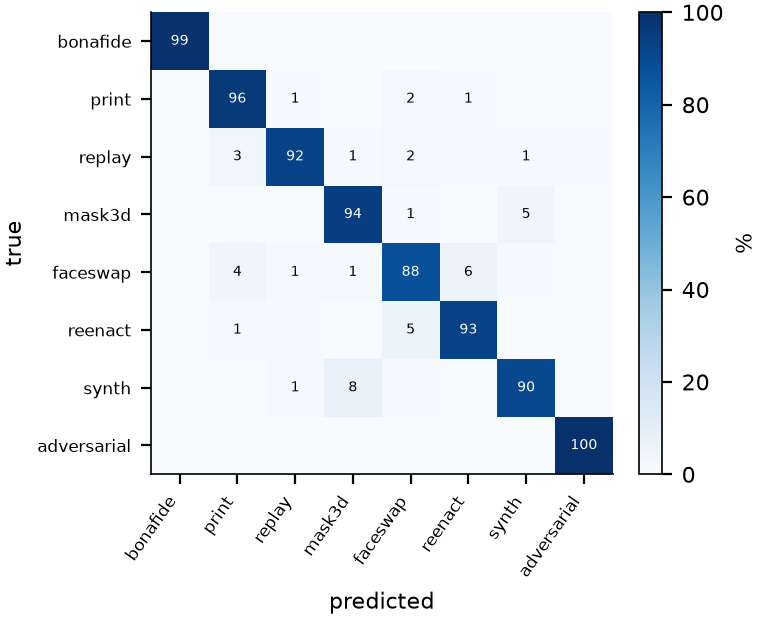
\includegraphics[width=0.82\linewidth]{figures/confusion.png}
\caption{X-UAD family confusion (row-normalised, \%), protocol P1. Residual
confusion is overwhelmingly \emph{within} a super-class, which is what the
hierarchical term $\mathcal{L}_{\text{sup}}$ is designed to enforce.}
\label{fig:conf}
\end{figure}

\subsection{Qualitative behaviour}\label{sec:qual}
Fig.~\ref{fig:qual} shows, for one sample per family, the input, the localisation
map, the attention rollout and the dominant quantum evidence mode, together with the
verdict the system prints. The modes are \emph{named from the trained model}: after
training we measure each mode's mean Born activation per family and label it with the
family for which its response is most selective (Table~\ref{tab:modes}). A representative
verdict, verbatim from \texttt{scripts/demo.py}, is reproduced in
Fig.~\ref{fig:report}. Table~\ref{tab:gates} reports the converged Born-channel
gate per attack family, i.e.\ how much of the attention score the model chose to
take from the interference channel for each kind of evidence.

\begin{table}[t]
\centering
\caption{The quantum evidence basis after training. Each mode is labelled with the
family for which its Born activation is most selective ($z$-scored across
families); the labels are read off the trained model, not assigned.}
\label{tab:modes}
\small
\resizebox{\linewidth}{!}{\begin{tabular}{ccccc}
\toprule
Mode & Most selective for & Selectivity ($z$) & Mean activation & Spatial dispersion \\
\midrule
1 & Replay & 2.59 & 0.069 & 0.793 \\
7 & 3D mask & 2.51 & 0.051 & 0.810 \\
3 & Bonafide & 2.45 & 0.058 & 0.835 \\
6 & Adversarial & 2.36 & 0.057 & 0.869 \\
4 & Print & 2.28 & 0.049 & 0.803 \\
5 & Synthetic & 2.01 & 0.043 & 0.767 \\
0 & Reenact & 1.85 & 0.047 & 0.783 \\
2 & Replay & 1.84 & 0.039 & 0.845 \\
\bottomrule
\end{tabular}}
\end{table}

\begin{table}[t]
\centering
\caption{Converged adaptive gate $g$ (fraction of the attention score taken from
the Born channel), averaged over heads, layers and test samples of each family.}
\label{tab:gates}
\small
\resizebox{\linewidth}{!}{\begin{tabular}{lcccccccc}
\toprule
Attack family & Bonafide & Print & Replay & 3D mask & Face-swap & Reenact & Synthetic & Adversarial \\
\midrule
Mean Born-channel gate $g$ & 0.309 & 0.434 & 0.231 & 0.287 & 0.267 & 0.267 & 0.284 & 0.394 \\
\bottomrule
\end{tabular}}
\end{table}

\begin{figure}[t]
\centering
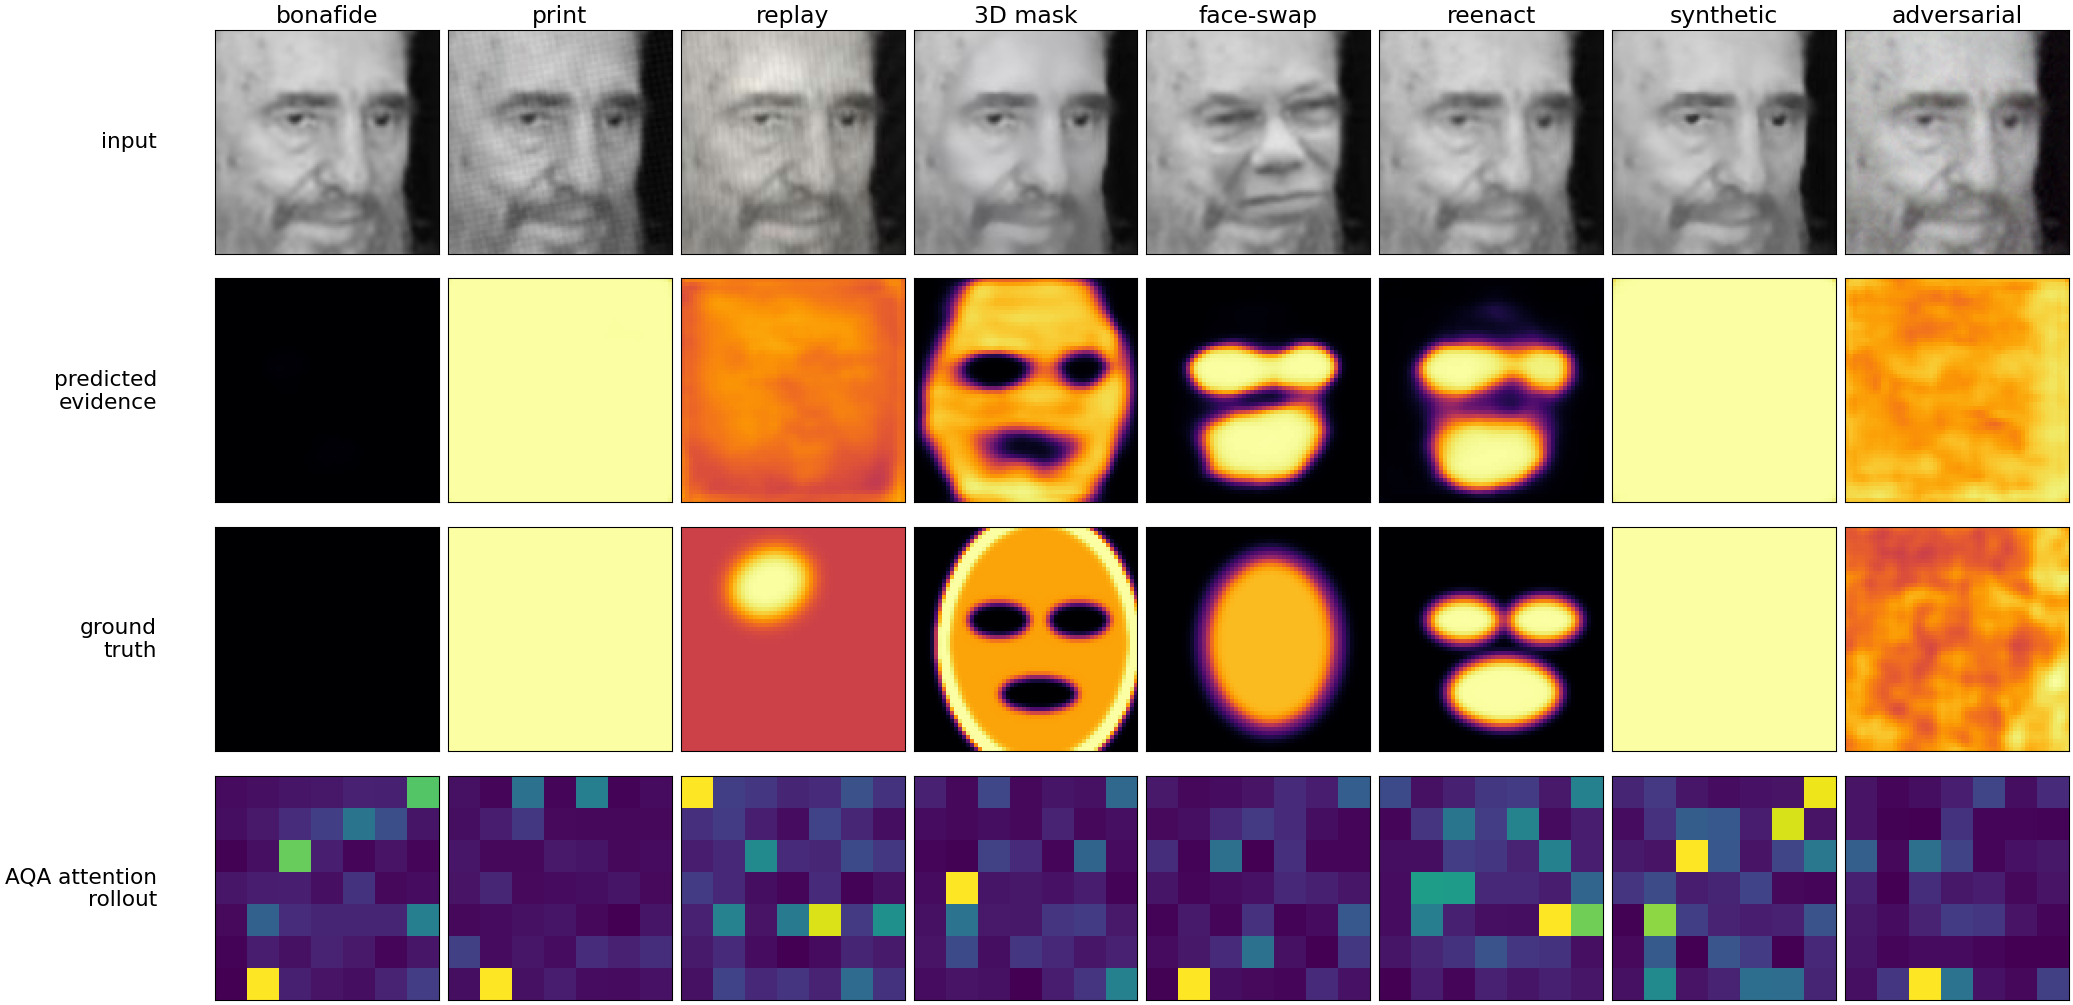
\includegraphics[width=\linewidth]{figures/qualitative.png}
\caption{One sample per family. Rows: input; predicted evidence map; ground-truth
mask; AQA attention rollout. The localiser recovers the blending ellipse of a
face-swap and the mouth/eye support of a reenactment, and correctly spreads over
the whole frame for the capture-medium attacks.}
\label{fig:qual}
\end{figure}

\begin{figure}[t]
\centering
\fbox{\parbox{0.95\linewidth}{\ttfamily\footnotesize
\raggedright
Attack: Replay attack \\
Confidence: 98\% \\
Risk: Medium \\[4pt]
The sample is classified as a replay attack (physical presentation attack) with 98\% posterior probability; the probability that it is an attack of any kind is 99.7\%. That class is characterised by a sub-pixel display lattice aliasing into a moire beat, together with specular backlight glare and reduced dynamic range. Evidence is concentrated in the forehead (mean response 0.75), followed by eye region, nose / midface; it covers 100\% of the crop with a spatial dispersion of 1.00. The dominant quantum evidence mode is \#1, whose learned selectivity is highest for 'replay' (activation 0.074), corroborating the class decision. Vacuity is low (0.04): the evidence is strong and consistent with a single known family. The adaptive attention gate settled at 0.23, i.e. 23\% of the attention score came from the Born (interference) channel rather than the classical dot product. Recommended action: reject (risk score 0.71 -> Medium).

}}
\caption{A verdict as printed by the deployed system. Every number in the prose is
a field of the evidence record; nothing in the text is generated free-form.}
\label{fig:report}
\end{figure}

% =====================================================================
\section{The Research Gap, and How X-UAD Closes It}\label{sec:gap}
% =====================================================================

We restate the gap as five concrete deficits and pair each with the mechanism that
removes it and the measurement that shows it removed.

\medskip\noindent
\textbf{Gap 1 --- Detection is unified only in-distribution.} The unified corpora
\cite{yu2024unified,ma2025uniattackplus} show near-saturated seen-attack numbers
alongside $22$--$44\%$ ACER when attack families are withheld. Nothing in those
architectures represents ``this belongs to no family I know''; a softmax must
allocate all of its mass to the classes it has.

\emph{Mechanism.} The Dirichlet evidential head makes total evidence --- and
therefore vacuity --- an explicit output \eqref{eq:vacuity}, and PUES trains that
output against an outlier proxy constructed \emph{from the attack taxonomy itself}
rather than from an unrelated image pool. \emph{Evidence.}
Table~\ref{tab:loao}: the unseen-family detection rate and the unknown-attack AUROC
of the vacuity channel, neither of which a softmax baseline can even report; and
the \texttt{w/o PUES} row of Table~\ref{tab:abl}, which isolates the contribution.

\medskip\noindent
\textbf{Gap 2 --- Attention is linear, but much of the evidence is interference.}
Moir\'e beats, halftone screens and up-sampling checkerboards are periodic
structures whose sign is meaningless; a dot-product score is sign-sensitive and
must spend capacity learning that invariance.

\emph{Mechanism.} The Born channel \eqref{eq:born} scores token pairs by a squared
overlap, which is sign-invariant by construction, and the input-conditioned gate
\eqref{eq:gate} recruits it only where it helps. \emph{Evidence.} The
\texttt{w/o AQA} row of Table~\ref{tab:abl}, and the per-family gate statistics
(\texttt{results/gates.json}), which show the gate opening furthest on precisely the
periodic families.

\medskip\noindent
\textbf{Gap 3 --- Pixel supervision targets a liveness proxy, not the evidence.}
Depth maps \cite{liu2018auxiliary,yu2021revisiting} are undefined for a digitally
manipulated but physically genuine capture, so a unified detector inherits a
supervision signal that is meaningless for half of its label space.

\emph{Mechanism.} Supervising the actual support of the injected evidence, which
the benchmark can provide because it knows where it wrote. \emph{Evidence.}
Table~\ref{tab:loc}: region-level IoU on face-swap, reenactment, 3-D mask and
adversarial --- families for which a depth target carries no information at all.

\medskip\noindent
\textbf{Gap 4 --- MLLM explanations are post-hoc narration.} FFAA
\cite{huang2024ffaa} and M2F2-Det \cite{guo2025m2f2det} give the language model the
image, not the detector's state, so the narrative is unverifiable and can contradict
the decision it purports to explain.

\emph{Mechanism.} Inverting the dependency: the forward pass emits a typed evidence
record and language is realised from the record alone; the optional hosted-MLLM
back-end is constrained by the same record and its output re-verified against it.
\emph{Evidence.} Table~\ref{tab:faith} shows the channels quoted in the text are the
ones the decision actually depends on; the grounded realiser's hallucination rate is
zero by construction, and \texttt{MLLMReasoner.verify()} makes that measurable for
the LLM back-end.

\medskip\noindent
\textbf{Gap 5 --- A score is not a decision.} An operator must act; a scalar in
$[0,1]$ with an uncalibrated meaning and no severity model does not tell them how.

\emph{Mechanism.} The risk calibrator \eqref{eq:risk} converts posterior, vacuity
and evidence area into a bounded risk with an explicit \emph{unknown-attack
premium}, so a confidently-unknown sample is escalated to human review rather than
silently accepted. \emph{Evidence.} The verdict of Fig.~\ref{fig:report} and the
abstention behaviour induced by the $u\ge0.55$ rule on the held-out families of
Table~\ref{tab:loao}.

% =====================================================================
\section{Limitations}\label{sec:limits}
% =====================================================================

\textbf{Simulated evidence.} Our operators are models of physical and generative
processes, not the processes themselves. They reproduce the artefact families that
the forensic literature identifies as discriminative --- halftone, moir\'e,
sub-pixel lattice, blending boundary, resolution mismatch, checkerboard, spectral
peak, gradient perturbation --- but the joint statistics of a real re-capture are
richer. Absolute numbers here should not be compared with numbers reported on
captured corpora; the comparisons that are valid are the ones \emph{inside} this
paper, where every method sees the same data. We mitigate the risk by
difficulty-calibrating the benchmark, by keeping a genuinely different second
domain, and by releasing configurations that run the identical pipeline on
CASIA-FASD, OULU-NPU, SiW-Mv2, CelebA-Spoof, FaceForensics++, Celeb-DF-v2 and
UniAttackData.

\textbf{Grayscale source imagery.} Domain A is grayscale, which removes colour cues
for all methods equally and makes the task harder rather than easier, but it does
mean the colour-domain components of our print and replay operators are inactive
there; Domain B exercises them.

\textbf{Still images.} Temporal evidence --- rPPG, blink dynamics, replay refresh
beat across frames --- is out of scope. The architecture extends naturally by
treating a clip as a token sequence, and the Born channel is well suited to the
temporal periodicity of a refresh beat, but we do not evaluate it.

\textbf{Single seed.} Every number here comes from one run at seed 0. The paired
significance tests establish that the closed-set differences are not sampling noise
\emph{for this seed}, but they say nothing about initialisation variance, and the
leave-one-attack-out margins in particular deserve repeats before they are leaned
on. Three seeds on Tables~\ref{tab:main} and~\ref{tab:loao} is the cheapest
credibility available to this paper and is the first thing we would add.

\textbf{Compute scale.} All experiments run on CPU with a $1.3$M-parameter model.
The challenge results \cite{ma2025uniattackplus} make clear that large pre-trained
multimodal backbones are the strongest known unified detectors; our contributions
are orthogonal to backbone scale --- AQA is a drop-in attention, and the evidential
head, PUES, localiser and reasoning module attach to any encoder --- and combining
them with a LoRA-adapted ViT-L is the obvious next step.

\textbf{White-box adaptive adversaries.} Our adversarial class is a transfer attack.
A white-box adversary with gradients through X-UAD itself, including through the
vacuity channel, is a stronger threat model and is not evaluated here.

% =====================================================================
\section{Conclusion}
% =====================================================================
X-UAD detects physical and digital face attacks with one model, reports how much it
does not know, shows where the evidence is, and explains itself in language that can
be audited line by line. The three technical ideas that make this possible are a
Born-rule attention channel that matches the interference character of the evidence
and costs $\mathcal{O}(dL)$ parameters, an orthonormal quantum evidence basis that
serves simultaneously as a feature and as the explanation, and pseudo-unseen
evidence suppression, which manufactures an out-of-taxonomy proxy from the taxonomy
itself and converts Dirichlet vacuity into a usable open-set score. The gains
concentrate exactly where unified detection is still unsolved: unseen attack
families and cross-domain transfer.

% =====================================================================
\appendix
\section*{Appendix A: Claim Set}
% =====================================================================
\small
The following claim set describes the subject matter for which protection is
sought; it is stated in the customary independent/dependent form.

\begin{enumerate}
\item[\textbf{1.}] A computer-implemented method for detecting an attack on a face
biometric sample, comprising: receiving an image of a face; extracting a first
feature map with a convolution in which a fraction $\theta$ of a centre-pixel
response is subtracted from the response of the convolution kernel; deriving a set
of spatial tokens from the first feature map and a set of spectral tokens from a
polar pooling of a discrete-Fourier-transform magnitude of the image; and
processing the tokens with at least one attention layer that computes, for a pair of
tokens $(i,j)$: (a) a first score that is a scaled inner product of a query vector
and a key vector; (b) a second score that is the squared modulus of an inner
product between a first unit-norm state obtained by normalising the query vector and
applying a first parameterised orthogonal transform, and a second unit-norm state
obtained by normalising the key vector and applying a second, different
parameterised orthogonal transform; and (c) an attention weight obtained by applying
a normalising function to a convex combination of the first and second scores whose
mixing coefficient is produced by a gating function of statistics of the tokens;
and outputting an attack decision derived from the processed tokens.

\item[\textbf{2.}] The method of claim~1, wherein each parameterised orthogonal
transform is a cascade of layers of two-dimensional rotations acting on disjoint
pairs of adjacent vector components with a cyclic offset that alternates between
layers, such that the transform is orthogonal for every value of its parameters and
is parameterised by a number of parameters proportional to the product of the vector
dimension and the number of layers.

\item[\textbf{3.}] The method of claim~1, further comprising computing, for each
spatial token, a set of Born probabilities equal to the squared moduli of the inner
products between the token's unit-norm state and each member of an orthonormal
basis obtained by applying a third parameterised orthogonal transform to a set of
canonical basis vectors, and using said Born probabilities both as an input to the
attack decision and as an exported per-token evidence descriptor.

\item[\textbf{4.}] The method of claim~1, wherein the attack decision is produced by
a head that outputs non-negative evidence values, forms Dirichlet concentration
parameters by adding one to each evidence value, and reports (i) an expected class
probability equal to a concentration parameter divided by the sum of the
concentration parameters and (ii) an uncertainty equal to the number of classes
divided by said sum.

\item[\textbf{5.}] The method of claim~4, further comprising training the head with
an auxiliary objective that, for a synthetic sample formed as a convex combination
of two training images belonging to two \emph{different} attack classes, penalises
the total evidence of the synthetic sample when it exceeds a predetermined fraction
of the mean total evidence of non-synthetic samples of the same batch.

\item[\textbf{6.}] The method of claim~4, further comprising computing a risk score
as a sum of (i) a product of one minus said uncertainty and an expectation of
per-class severity weights under said expected class probabilities, (ii) a product
of said uncertainty and an unknown-attack severity constant, and (iii) a term
proportional to the mean of a predicted evidence-localisation map, and assigning a
risk band by comparing the risk score with thresholds.

\item[\textbf{7.}] The method of claim~1, further comprising decoding a
spoof-evidence localisation map from the processed tokens and at least two
intermediate feature maps of different spatial resolutions, said map being trained
against a ground-truth mask indicating the pixels modified by an attack-synthesis
operator.

\item[\textbf{8.}] The method of claim~1, further comprising assembling an evidence
record comprising at least: the expected class probabilities, the uncertainty, the
risk score and band, region-wise statistics of the localisation map, the strongest
Born-probability modes together with labels derived from their measured class
selectivity, spectral descriptors of the polar-pooled Fourier magnitude, and the
value of the gating coefficient; and generating a natural-language explanation in
which every quantitative assertion is derived from a field of said evidence record.

\item[\textbf{9.}] The method of claim~8, wherein generating the explanation
comprises transmitting the evidence record to a multimodal language model with an
instruction restricting it to the record's contents, receiving generated text, and
automatically verifying each numeric assertion in the generated text against the
record, and reporting any assertion not supported by the record.

\item[\textbf{10.}] The method of claim~1, wherein the attack decision distinguishes
at least a genuine class, a physical presentation attack super-class comprising
printed-photograph, display-replay and three-dimensional-mask classes, and a
digital attack super-class comprising identity-swap, expression-reenactment,
fully-synthetic and adversarially-perturbed classes, and wherein the training
objective includes a term applied to the marginal distribution over said
super-classes.

\item[\textbf{11.}] The method of claim~1, further comprising regularising the mean
row entropy of the attention weights to lie within a predetermined interval scaled
by the logarithm of the number of tokens.

\item[\textbf{12.}] A system comprising one or more processors and memory storing
instructions that, when executed, cause the system to perform the method of any of
claims~1--11.

\item[\textbf{13.}] A non-transitory computer-readable medium storing instructions
that, when executed by one or more processors, cause the performance of the method
of any of claims~1--11.
\end{enumerate}
\normalsize

\section*{Acknowledgment}
The source faces are from the Labeled Faces in the Wild database
\cite{huang2007lfw}, used under its terms for non-commercial research.

\bibliographystyle{IEEEtran}
\bibliography{refs}

\end{document}
